% Created 2020-08-20 gio 13:13
% Intended LaTeX compiler: pdflatex
\documentclass[a4paper,12pt]{article}
\usepackage[utf8]{inputenc}
\usepackage[T1]{fontenc}
\usepackage{graphicx}
\graphicspath{ {./images/} }
\usepackage{grffile}
\usepackage{longtable}
\usepackage{wrapfig}
\usepackage{rotating}
\usepackage[normalem]{ulem}
\usepackage{amsmath}
\usepackage{textcomp}
\usepackage{amssymb}
\usepackage{capt-of}
\usepackage{hyperref}
\usepackage[margin=1in]{geometry}
\usepackage{multirow}
\usepackage{booktabs}
\usepackage{setspace}

\newcommand*\BitAnd{\mathbin{\&}}
\newcommand*\BitOr{\mathbin{|}}
\newcommand{\BitNeg}{!}
\newcommand*\ShiftLeft{\ll}
\newcommand*\ShiftRight{\gg}
\renewcommand{\arraystretch}{1.0}
\setlength{\parskip}{1em}
\setlength{\abovetopsep}{0.5em}
%\renewcommand{\baselinestretch}{1.3}
\setstretch{1.4}
\newcommand{\cltloc}{CLTLoc}
\newcommand{\aez}{ae2sbvzot}
%\author{Robert Smith}
%\date{\today}
%\title{SMT Translation}
\begin{document}
\title{Improved Verification of Networks of Timed Automata}
  \begin{titlepage}
	\bfseries{
		\begin{center}
			{\Large Politecnico di Milano\\}
			{\large
			Scuola di Ingegneria Industriale e dell'Informazione\\
			Master Degree in Computer Science and Engineering\\
			Dipartimento di Elettronica, Informazione e Bioingegneria\\}
		\end{center}
	
	}
	\vspace{1.0cm}
	\begin{figure}[h]
		\centering
		
\includegraphics[width=10cm]{./frontpage/logo.png}
	\end{figure}
	\vspace{0.5cm}
	\begin{center}
		\textsc{\huge Improved Verification of Networks of Timed Automata}
		%
	\end{center}
	\vspace{2cm}
	\begin{flushleft}
		\texttt{Supervisor: Prof. Pierluigi San Pietro}%\\
		%Co-supervisor: Doc. Mersedeh Sadeghi}
	\end{flushleft}
	\vspace{2cm}
	\begin{flushright}
		Tesi di laurea di:\\
		Robert Lawrence Smith\ \ Matr. 914634
	\end{flushright}
	\vspace{1cm}
	\begin{center}
		Academic Year: 2019-2020 %check this
	\end{center}
\end{titlepage}


%\maketitle
\tableofcontents
\listoffigures
\listoftables

\section{Introduction}\label{introduction}
\iffalse
Timed Automata are a commonly used representation for modeling the behavior of
systems with real-time semantics.


Current examples of TA bounded model checkers include XX, YY, and de facto
standard Uppaal. TACK is a tool focused on allowing for the expression of TA
properties in Metric Interval Temporal Logic, a rich \ldots{}

TACK translates both the TA and the property to be verified into CLTLoc.
Constraint Linear Temporal Logic (over clocks) is a variant of

Zot

Sbvzot is a very successful solver which takes advantage of bit vector logic\ldots{}

To further improve the performance of TACK, we wish to directly translate the
network of timed automata into the SMT-LIB format, skipping the intermediate
CLTLoc representation. While CLTLoc is an elegant expressive language, there is
a significant overhead in
\fi
\section{Preliminaries}\label{prelims}
\subsection{Timed Automata}\label{timed-automata}

Timed Automata are a useful model for many interactions that require precise
timing mechanisms. Each Timed Automaton has a set of states, one of which is
active at any given moment, much like a Finite State Machine. Also like a FSM, a
Timed Automaton has a set of transitions that allow it to move between different
states. However these transitions come with powerful timing properties that
allow for finer control over the progression of the automata. Included with our
automata is a network of clocks and integer variables. Clocks progress as time
passes, and can be used alongside variables as prerequisites for taking
transitions and remaining in states. Transitions can also reset these clocks
(and assign new values to variables), allowing for communication and shared
state between different Timed Automata. For explicit synchronization, we
define a set of synchronization primitives that can be used to coordinate
transitions between different automata. Finally, states can be labeled with
atomic propositions, to aid in defining model properties that we will then
verify over the network. To help concretize this concept, we will introduce a
simple Timed Automaton, which will be used throughout this paper to help
visualize important concepts.

%\begin{figure}[h]
%    \centering
%    \def\svgwidth{0.50\columnwidth}
%    \input{images/example-min.pdf_tex}
%    \caption{Simple TA example}
%    \label{fig:example-min}
%\end{figure}
\begin{figure}[h]
  \centering
  \includegraphics[width=0.5\textwidth]{minTA-blank}
  \caption{A basic Timed Automaton}
  \label{fig:example-blank}
\end{figure}

As we can see in figure \ref{fig:example-blank}, Timed Automata have many
similarities with Finite State Machines and other automata. For a given
automaton $\mathcal{A}_{i}$, the example TA consists of a finite set of states
$Q_{i} = \{q_{1},q_{2},q_{3}\}$, and a finite set of transitions
$T_{i} = \{t_{1},t_{2},t_{3},t_{4}\}$. Like a finite state machine, at a given
moment in time there is one state that is ``active''. The TA can take
transitions that may change its state, with the condition that the source of the
transition must be the currently active state. We denote the source state of a
transition $t$ as $t_{-}$, and the destination state as $t_{+}$. As an example,
if the current active state is $q_{1}$, then either $t_{1}$ or $t_{2}$ can be
taken. Although not shown in this example, the source and destination state of a
transition may be the same state, and there may be multiple transitions with
identical source states and identical destination states.

In addition to states and transitions, TA are enriched with clocks and bounded
integer variables. Clocks are variables over $\mathbb{R}_{\geq 0}$ that increment with the
passage of time. Their ability to continuously change value is fundamental to
the ability of timed automata to model time-sentisive and real-time systems.
Meanwhile the bounded integer variables do not change value on their own, and
have to be explicitly modified by the TA.

\begin{figure}[h]
  \centering
  \includegraphics[width=0.6\textwidth]{minTA-big}
  \caption{A Timed Automaton with clock $x$ and variable $n$.}
  \label{fig:example-big}
\end{figure}

We can now show how these values are used and manipulated by a timed automaton.
Figure \ref{fig:example-big} shows the same example TA modified with transition
guards, transition assignments, and state invariants. Transition guards are
conditions over either clocks or variables that prevent the associated
transition from being taken when they do not evaluate to true. As an example,
transition $t_{2}$ can only be taken when the value of clock $x$ is greater than
$5$. Assignments on the other hand modify the value of a clock or variable
\emph{after} the transition has been taken. For example, it is perfectly valid
for transition $t_{2}$ to be taken when $x=6$, even though the assignment
$x=0$ resets the value of $x$ to $0$, which is smaller than the value
accepted by the transition guard $x>5$. Variables can be assigned to any value,
while clocks can only be reset to $0$. The third feature to mention are the
state invariants. In our example there is only one, $x<2$ which is associated
with state $q_{2}$. When a state is active, its invariant (if any) is required
to be true. The invariant attached to $q_{2}$ requires the TA to `leave' state
$q_{2}$ before clock $x$ reaches a value of $2$.


In addition to clocks and variables, TA also offer a powerful synchronization
mechanism for different automata in the same network to coordinate. Any
transition may contain a synchronization event of the form
$\{channel \times sync\}$, where $channel$ can be any symbol and
$sync \in \{!,?,\#,@\}$. Two different timed automata can synchronize their
transitions by labelling them with the same synchronization channel, and using
the actions to describe the type of synchronization desired.

\begin{table}
  \centering
  \begin{tabular}{l p{0.7\textwidth}}
    \textbf{Type} & \textbf{Synchronization Semantics} \\
    \midrule
    One-to-one & Whenever a TA $\mathcal{A}_{i}$ takes a transition with a
                 syncronization event $\alpha{!}$, there exists exacty one
                 $\mathcal{A}_{j}$, $i\neq j$, such that in the same instant
                 $\mathcal{A}_{j}$ has an active transition $t'$ with the
                 synchronization event $\alpha{?}$, and vice versa. \\
    \midrule
    Broadcast &  Whenever a TA $\mathcal{A}_{i}$ takes a transition with a
                synchronization event $\alpha\#$, every other TA
                $\mathcal{A}_{j}$ must not simultaneously take a transition with
                the same event, and must either simultaneously take a transition
                labelled with $\alpha@$, or there must not exist a transition
                $t' \in \mathcal{A}_{j}$ such that $t_{-}$ is the currently
                active state, $\alpha@$ is the synchronization event, and the
                clock and variable guards of $t'$ are satisfied.
    \\
    \midrule
  \end{tabular}
  \caption{Supported Synchronization Events}
  \label{table:sync-def}
\end{table}

As shown in table \ref{table:sync-def}, two types of synchronization are
defined. The first type is one-to-one synchronization, which has two associated
operators, one signifying one-to-one `send' (${!}$), and the second for
one-to-one receiving (${?}$). A transition labelled with $\alpha{!}$, for some
channel $\alpha$, can only be fired if at the same moment in time, another TA
takes a transition labelled with the $\alpha{?}$ event. The second type of
synchronization available is termed `broadcast' synchronization, and again we
have two operators, broadcast-send ($\#$) and broadcast-receive (${@}$). Like
one-to-one synchronization, for a given channel $\alpha$ there can only be one
active transition with the event $\alpha\#$, however the difference is that
there can be 0,1, or multiple automata that sync using broadcast-receive at
once. In addition, each automaton is \emph{required} to perform a broadcast-sync
if it is able to, meaning that there exists a transition $t$ such that $t_{-}$
is the currently active state, and all guards of the transition are satisfied.


With the basic concepts introduced, we will formally define the Timed Automata
discussed in this paper. Let \(AP\) be a set of atomic propositions, and let \(Act\) be a set of
synchronization events of the form $Act \subset \{channel \times sync\}$,
where channel is a set of symbols and $sync \in \{!,?,\#,@\}$. In addition we
define a null event \(\tau\). \(Act_{\tau}\) is the set \(Act \cup \{\tau\}\).
Let \(X\) be a finite set of clocks, and \(Int\) a finite set of integer-valued
variables. \(\Gamma(X)\) is the set of clock constraints, where a clock
constraint \(\gamma\) is a relation
\(x \sim c \BitOr \neg \gamma\BitOr \gamma \land \gamma\), where \(x \in X\),
\(\sim \in \{<,=\}\), and \(c \in \mathbb{N}\). \(Assign(X)\) is the set of
clock assignments, where each assignment has the form \(x {=} 0\), where
\(x \in X\iffalse{,\ c {\in} \mathbb{Z}^+}\fi\). \(Assign(Int)\) is a set of
variable assignments of the form \(y := exp\), where
\(exp := exp + exp\BitOr exp - exp\BitOr n\BitOr c\),
\(n \in Int\) and \(c \in \mathbb{Z}\). \(\Gamma(Int)\) is the set of integer
variable constraints, where a variable constraint \(\gamma\) is defined as
\(\gamma := n \sim c\BitOr n \sim n'\BitOr \neg \gamma\BitOr \gamma \land \gamma\),
where \(n\) and \(n'\) are integer variables, \(c \in \mathbb{Z}\), and
\(\sim \in \{<,=\}\). A Timed Automaton with variables is defined as the tuple
\(\mathcal{A} = \big \langle AP,X, Act_{\tau}, Int, Q, q^0, v_{var}^0, Inv, L, T \big \rangle\).
In this tuple \(Q\) is the finite set of states of the timed automaton,
\(q^0 \in Q\) is the initial state of the TA,
\(v_{var}^{0} : Int \rightarrow \mathbb{Z}\) is a function providing initial
values for each of the variables, and \(Inv : Q \rightarrow \Gamma(X)\) is a
function assigning each state to a (possibly empty) set of clock constraints.
The labeling function \(L: Q \rightarrow \mathcal{P}(AP)\) assigns each state to
a subset of the atomic propositions. Each transition \(t \in T\) has the form
\(t = \big \langle Q \times Q \times Act_{\tau} \times \Gamma(X) \times \Gamma(Int) \times \mathcal{P}(Assign(X)) \times \mathcal{P}(Assign(Int)) \big \rangle \),
consisting of a source and destination state, an action, a set of clock and
variable guards, a set of clocks to be reset when the transition fires, and a
set of variables to assign values to. To refer to the components of a transition
we will use \(t_-\) and \(t_+\) to refer to the source and destination states
respectively, as well as
\(t_\epsilon, t_{\gamma_c}, t_{\gamma_v}, t_{a_c}, t_{a_v}\) to refer to the
event, clock constraints, variable constraints, clock assignments, and variable
assignments respectively.

A network of Timed Automata is a finite list of timed automata \(\mathcal{A} =
[\mathcal{A}_1, \mathcal{A}_2, \ldots \mathcal{A}_N]\). Timed Automata in the
same network can refer to common clocks, variables, and synchronization channels
to coordinate their actions. To simplify the notation we will use the symbols
\(T\), \(X\), \(Int\), and \(Act/Act_{\tau}\) to refer to the union of the respective
sets of each individual timed automaton in the network. When necessary to refer
to the properties of one timed automaton in particular, we will append a
numerical subscript to the set in question, for example \(X_i\) to refer to the
clocks used by the specific timed automaton \(\mathcal{A}_{i} \in \mathcal{A}\).

\subsection{Bounded Model Checking}\label{bounded-sat}

% TODO: define trace, create graphic showing trace progression
%       define liveness, 2 types of edges
%       (cut and paste existing sections on this topic from later sections)
%       then move on to the TACK section
%

Bounded Model Checking refers to the problem of evaluating if a given network of
timed automata satisfies a given model, or property. To perform this evaluation,
the TA network along with the property to be evaluated are transformed into a
form acceptable by a Satisfiability Modulo Theories, or SMT solver. The solver
then searches all possible executions of the system to determine if the property
is satisfied. Before we can discuss this process, we must describe what we mean
by an execution of a network of timed automata.

At a given position in time, the TA network can be described by the currently
active states, as well as the values of the clocks and integer variables.
Because the execution of a TA is a series of instantaneous state transitions,
interspersed throughout time, we can represent a TA execution as a series of
`snapshots' showing these moments of transitions. In order to achieve this
representation, we use the concept of a trace. A trace consists of an infinite
sequence of \emph{time positions} $S = \{s_{0}s_{1}s_{2}\ldots\}$. Each time
position contains the active state of each timed automaton, the current values
of each clock and variable, the amount of time $\delta$ that will elapse before
the next position, and the transition to be taken by each timed automaton at the
next time position. For a given position we will use $l[i]$ and $t[i]$
to denote the active state and transition of automaton $\mathcal{A}_{i}$.

\begin{figure}[h]
  \centering
  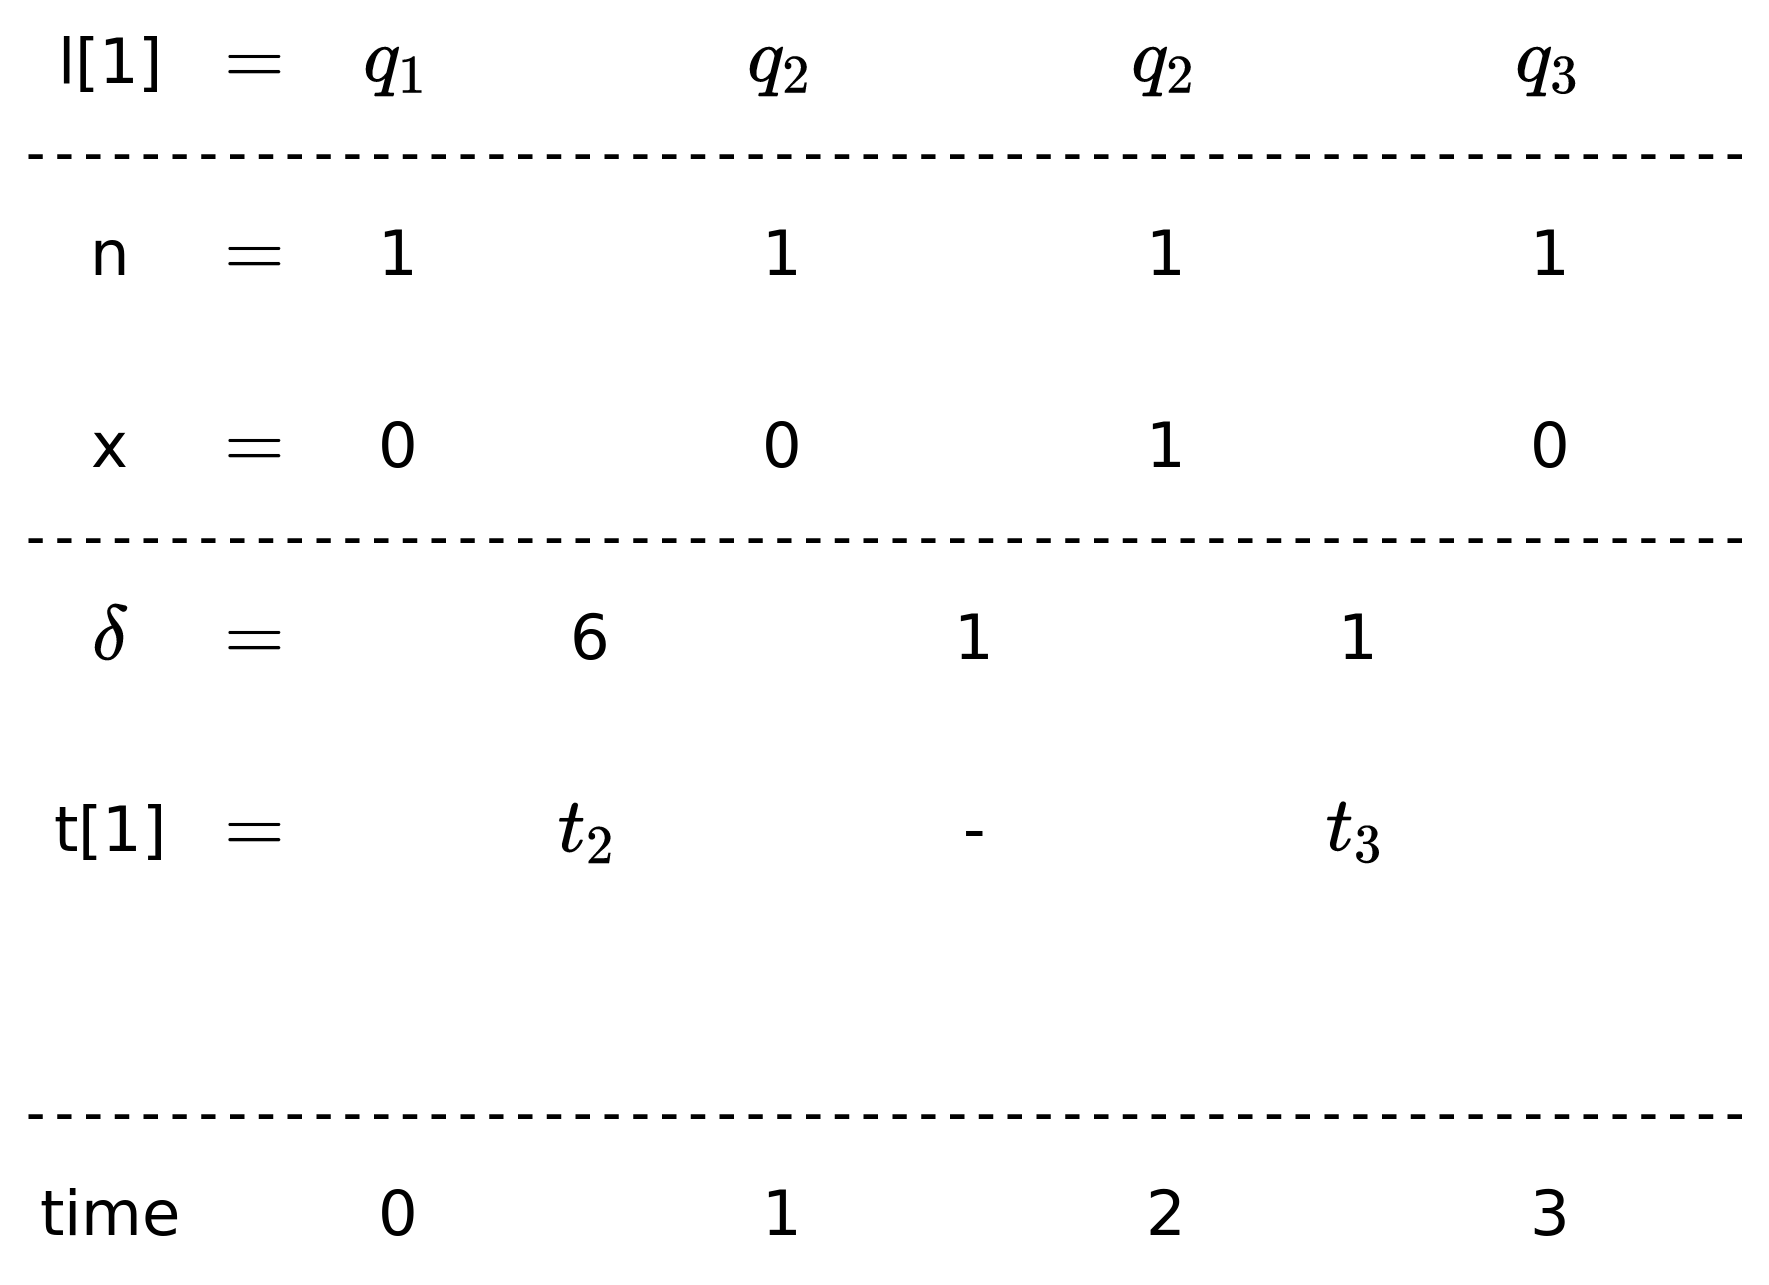
\includegraphics[width=0.6\textwidth]{trace-shift-min}
  \caption{An example trace through 4 positions.}
  \label{fig:trace-min}
\end{figure}

In figure \ref{fig:trace-min} we can see a trace of the Timed Automaton defined
in figure \ref{fig:example-big}, which has been given an index of 1. To prevent
the value of $t[i]$ being undefined at position $0$, the value of $t[i]$
corresponds to the transition taken in the following time position. However for
clarity in the traces shown here, the values of $t[1]$ have been shifted to the
right by one position, so that the active transition is lifted over the position
in time where the transition actually occurs. At the top of the trace $l[1]$
tracks the currently active state of the timed automaton. In this simple trace
the automaton begins in state $q_{1}$, transitions to $q_{2}$, remains in
$q_{2}$ for another position, and then transitions to $q_{3}$. Below the active
state we show the active values of both the variable $n$ and the clock $x$ at
the given positions. The value $\delta$ shows the amount of time that passes
between the current state, and the immediately following state.

One surprising observation is that the value of the clock $x$ does not seem to
change between positions $0$ and $1$, despite $\delta$ indicating that $6$ units
of time has passed. Recall that transition $t_{2}$ resets the value of the clock
$x$ to zero, and that the trace capture the values of clocks and variables
\emph{after} any assignments have been applied.

\begin{figure}[h]
  \centering
  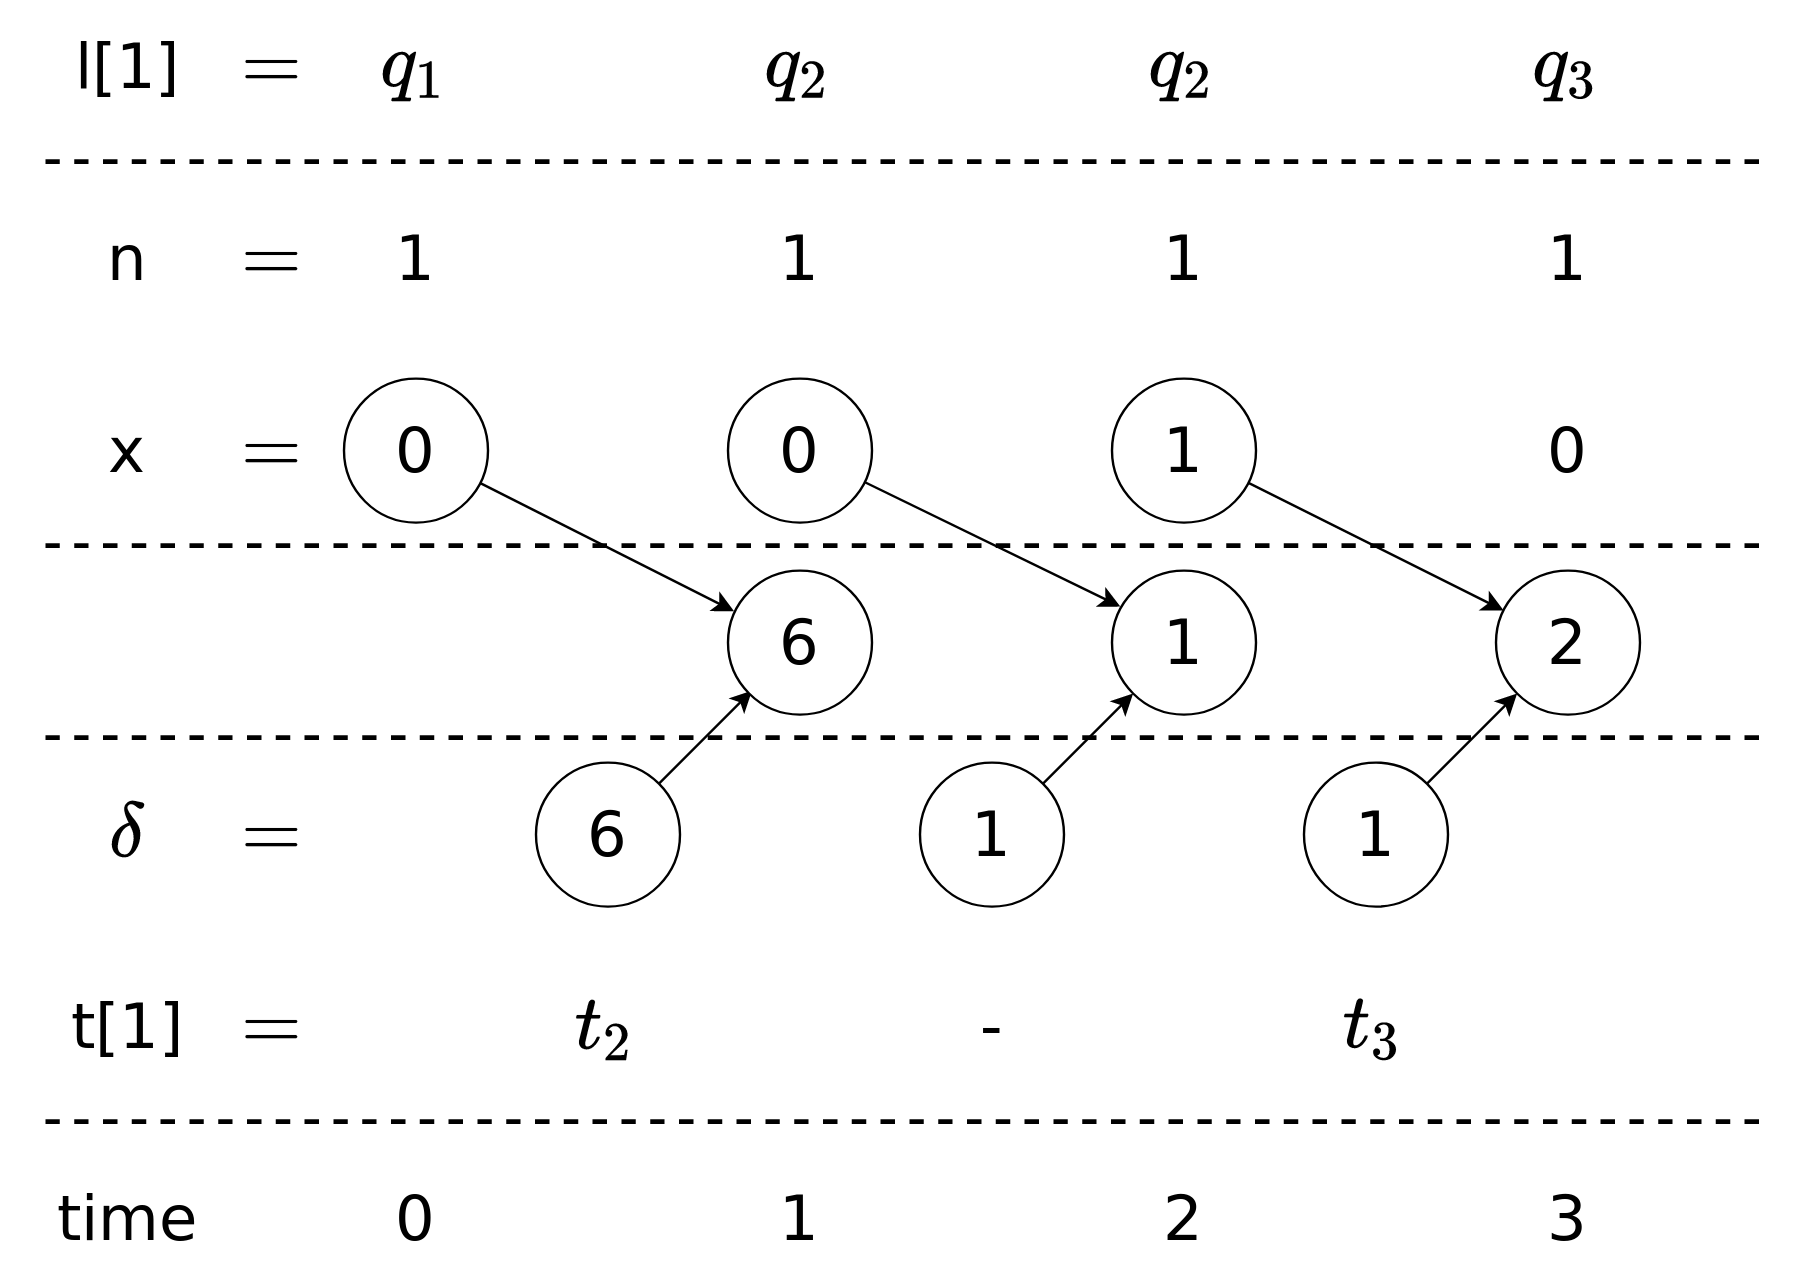
\includegraphics[width=0.6\textwidth]{trace-shift-delta}
  \caption{A trace highlighting the evaluation of a clock guard.}
  \label{fig:trace-delta}
\end{figure}

Figure \ref{fig:trace-delta} shows how we can compute the value of clock $x$ at
the moment of the transition, before the reset is applied. By combining the
values of $x$ and $\delta$, we obtain the value of $x$ that is used to determine
if the clock guard of transition $t_{2}$ is satisfied. We see that $x$ has a
value of 6, which satisfies the guard $x>5$.

Notice in the above trace the value of clock $x$ during the transition from
state $q_{2}$ to state $q_{3}$. State $q_{2}$ has an invariant requiring that
the value of clock $x$ be strictly less than $2$, however at the moment of
transition $x() + \delta() = 2$. Is this trace therefore illegal? This raises an
interesting question: at the moment of transition, what is the active state?
Possible answers could include the source state, the destination, both, or
neither. Different models of Timed Automata implement this
differently\cite{TODO-give-example}. In our model, the TA is always in exactly
one state at every instant in time. If at the moment of transition the TA
remains in the source state, the transition is said to be ``right-closed'' or
equivalently ``left-open'', because the interval of time that the TA spends in
\(t_{-}\) ends in a closed interval, while the inteval of time that the TA
spends in \(t_{+}\) begins in an open interval. Conversely if the TA is located
in the destination state at the moment of transition, we say that it is
``left-closed'', which also implies that it is right-open. Returning to our
example trace, if the timed automaton is not in state $q_{2}$ in the instance of
transition, then the strict inequality in the state invariant can be satisfied
with equality at the instance of transition, since the automaton is not actually
in that state at that final moment. To formalize this notion we introduce the
weak clock relation $\sim_{w}$, which is defined as follows:
\begin{align*}
  x \sim_{w} c  \iff & (x \sim c\ \lor\ x = c) \ \ \sim \in \{<,>,\leq,\geq\} \\
  x =_{w} c  \iff & false
\end{align*}
To make our trace more precise, we add for each TA $\mathcal{A}_{i}$ the term
$edge^{RC}[i]$, which is true at a given time position iff the currently active
edge is right-closed.

\begin{figure}[h]
  \centering
  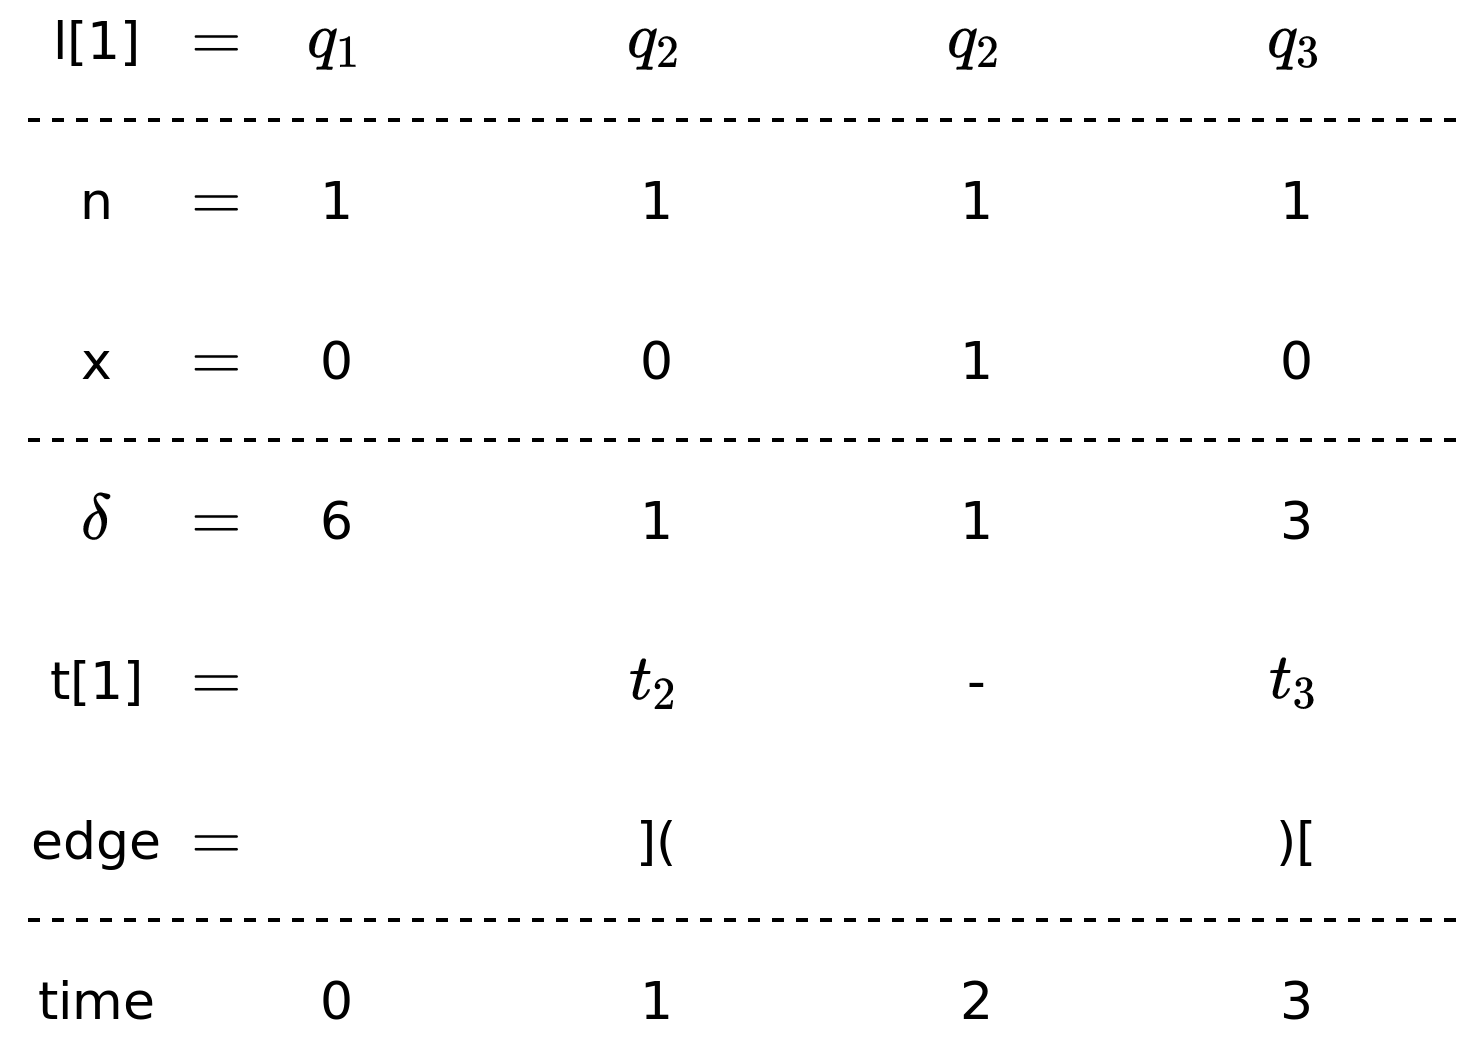
\includegraphics[width=0.6\textwidth]{trace-shift-full}
  \caption{An example trace with edge variable.}
  \label{fig:trace-full}
\end{figure}

Figure \ref{fig:trace-full} shows the same example trace as before, but with the
addition of the edge variable. Like the transitions, it is shifted to the right
by one position for ease of viewing. Notice that when transition $t_{3}$ is
taken, the edge is left-closed, as is required by the invariant. The value of
the edge variable is not shown during the null transition, however during a null
transition either value is equivalent.


When using Timed Automata to model real-time systems, a common desire is to
verify that every valid trace of the system obeys a given constraint, or
property. Problems of feasibility quickly arise however, due to the infinite
length of these traces. Bounded Model Checking is a process in which
timed automata traces of infinite length can be efficiently verified against a
property. Since TA traces are infinite in
length, we restrict ourselves to traces of the form
\(s_0 s_1\ldots s_{l-1}{(s_l s_{l+1}\ldots s_{k-1}s_k)}^\omega\). These
``lasso-shaped'' traces consist of an initial sequence of states up until
\(s_{l-1}\), followed by a loop that can be repeated an infinite amount of times
to form the full trace. Since the beginning of the loop is allowed to occur
anywhere within the sequence, the only variable is the number of distinct states
\(k\). Bounded Model Checking refers to checking if a given property is
satisfied over lasso-shaped traces of up to length \(k\).
The TA system along with the desired property are converted into a
format suitable for parsing by a SAT or SMT solver, which is then tasked
with finding a counterexample to the property. If a counterexample is
found, then there exists at least one trace that does not satisfy the provided
property. Otherwise, the property is said to have been verified over the TA
network up to the bound \(k\), as the solver has shown that no lasso-shaped
traces of length \(k\) exist that contradict the property.

\subsection{Constraint LTL Over Clocks}\label{cltloc}

\cltloc\ is a temporal logic that allows for the construction of formulas
defined over atomic propositions, clocks, and arithmetic variables. A clock is a
variable over \(\mathbb{R}_{\geq 0}\) whose value changes between LTL positions
to model the passage of time. Like clocks in timed automata, clocks can be
reset back to zero.

A formula in \cltloc\ consists of atomic propositions, clock formulas, and
formulas over integer variables, which are combined using the standard LTL
operators of \(\mathcal{X}\) (next) and \(\mathcal{U}\) (until), as well as the
derived operators \(\mathcal{G}\) (globally), \(\mathcal{F}\) (future), and
\(\mathcal{R}\) (release). A clock formula compares the value of the clock to a
given natural number, for instance \(x > 7\). A variable formula, on the other
hand, can compare not only individual variables but also arithmetic combinations
of variables. An example would be the expression \(b + c = 7\); \(b,c \in Int\).

Let \(X\) be a finite set of clocks and \(Int\) be a finite set of integer
variables. \cltloc\ formulas are defined as follows:
\[\phi := a \BitOr x \sim c \BitOr \exp \sim \exp \BitOr \mathcal{X}(n) \sim \exp \BitOr \phi \land \phi \BitOr \neg \phi \BitOr \mathcal{X}\phi \BitOr \phi \mathcal{U} \phi \]
Where \(a \in AP\), \(x \in X\), \(c \in \mathbb{N}\), \(n \in Int\), and
\(exp\) are arithmetic formulas over integer variables. As mentioned before,
clocks are special dense variables over \(\mathbb{R}_{\geq 0}\) that `progress'
between different LTL positions. To be more specific, each clock must either
increment between two adjacent time positions, or it must be reset. To maintain
a consistent view of time, we introduce
\(\delta: \mathbb{N} \rightarrow \mathbb{R}_{>0}\), which measures the amount of
time that elapses between two adjacent time positions. For a given clock
`valuation' \(\sigma: \mathbb{N} \times X \rightarrow \mathbb{R}_{\geq 0}\),
each clock \(x \in X\) must either obey the equivalence
\(\sigma(i,x) + \delta(i) = \sigma(i+1,x)\), or is reset, i.e.\
\(\sigma(i+1,x) = 0\). This ensures that all clocks progress at the same rate,
and we can use \(\delta(t)\) to calculate the amount of time elapsed between any
two positions.

\subsection{TACK \cltloc\ Translation}\label{prelim-tack}

The TACK\cite{tack20} tool developed by Menghi et al.\ converts Bounded
Satisfiability Checking problems into the CLTLoc language. TACK uses Metric
Interval Temporal Logic to specify the property to be checked for satisfiability,
which allows for more compact and powerful specifications of the desired
properties to be checked. Once the Timed Automata network and the MITL property
have been converted into CLTLoc, TACK then uses the tool Zot to convert this
intermediate representation of the problem into the SMT-LIB2 language, which is
supported by many modern SMT solvers. Zot was designed with a modular
architecture to allow for several different strategies and algorithms that can
be used to convert its input. Currently the most successful Zot plugin for
CLTLoc Bounded Model Checking is \aez. We will provide an overview of both
the TACK encoding of Timed Automata in CLTLoc and the ae2sbvzot translation of
CLTLoc into BitVector form.

\begin{table}
  \begin{tabular}{p{0.2\textwidth} p{0.7\textwidth}}
    \toprule
    \textbf{Type} & \textbf{Liveness Semantics} \\
    \midrule
    Strong transition liveness & Every TA will always transition at some point
                                 in the future. \\
    \midrule
    Weak transition liveness & At least 1 TA will always transition at some
                               point in the future. \\
    \bottomrule
  \end{tabular}
  \caption{Liveness Semantics}
  \label{table:liveness-def}
\end{table}


\begin{table}\label{tack-encoding}
  \centering
  % \setlength{\tabcolsep}{4pt}
  \aboverulesep=0ex
  \belowrulesep=0ex
  \renewcommand{\arraystretch}{1.2}
  \caption{TACK Encoding of an Automaton in CLTLoc}
  \begin{tabular}{c|c|c}
    \toprule
    \(\varphi_{1} := \underset{i \in [1,N]}{\bigwedge} (l[i] = 0)\) &
                                                                 \(\varphi_{2} := \underset{n \in Int}{\bigwedge} n = v_{var}^0 (n) \) &
                                                                                                                                     \(\varphi_{3} := \underset{i \in [1,N]}{\bigwedge} Inv(l[i])\) \\
    \midrule
    \(\varphi_{4} {:=} \underset{x \in X}{\bigwedge} (x_{0} {=} 0 \land x_{1} {>} 0 \land x_{v} {=} 0)\) &  \multicolumn{2}{c}{\( \varphi_{5}(j) {:=} \underset{x \in X}{\bigwedge} (x_{j} {=} 0) {\rightarrow} \mathcal{X}\left( (x_{(j{+}1){\mod 2}} = 0) \mathcal{R}\big( (x_{v}{=}j){\land}(x_{j}{>}0) \big) \right) \)} \\
    \midrule
    \multicolumn{3}{c}{\(\varphi_{6} := \underset{q \in \mathcal{Q}_{i}}{\underset{i \in [1,N]}{\bigwedge}} \bigg( \Big( l[i] = q \land t[i] = \sharp \Big) \rightarrow \mathcal{X} \Big( Inv(q) \land r_{1}(Inv(q)) \Big) \bigg) \)} \\
    \midrule
    \multicolumn{3}{c}{\( \varphi_{7} := \underset{t \in T_{i}}{\underset{i \in [1,N]}{\bigwedge}} t[i] = t \rightarrow \Big( l[i] = t_{-} \land \mathcal{X}(l[i] = t_{+}) \land \varphi_{\gamma_{c}} \land \varphi_{\gamma_{v}} \land \varphi_{\alpha_{c}} \land \varphi_{\alpha_{v}}  \land \varphi_{edge}(t_{-}, t_{+}, i) \Big) \)} \\
    \multicolumn{3}{c}{\( \varphi_{edge}(a,b,i) := \varphi_{\alpha](}(a,b,i) \lor \varphi_{\alpha)[}(a,b,i) \)} \\
  %  \multicolumn{3}{c}{\( \varphi_{\alpha](}(a,b,i) := Inv(a) \land r_{2}(Inv_{w}(b)) \land edge^{](}[i] \)} \\
    \multicolumn{3}{c}{\( \varphi_{\alpha)[}(a,b,i) := Inv_{w}(a) \land r_{2}(Inv(b)) \land \neg edge^{](}[i] \)} \\
    \midrule
    \multicolumn{3}{c}{\( \varphi_{8} := \underset{i \in [1,N]; q,q^{'} \in \mathcal{Q}_{i} | q \neq q^{'}}{\bigwedge} \bigg( \Big( (l[i] = q) \land \mathcal{X}(l[i] = q^{'}) \Big) \rightarrow \underset{t \in T_{i} | t_{-} = q, t_{+} = q^{'}}{\bigvee} (t[i] = t) \bigg) \)} \\
    \midrule
    \multicolumn{3}{c}{\( \varphi_{9} := \underset{x \in X}{\bigwedge} \bigg( \mathcal{X}(x_{0} = 0 \lor x_{1} = 0) \rightarrow \underset{t \in T_{i} | x \in t_{a_{c}}}{\underset{i \in [1,N]} {\bigvee}} t[i] = t \bigg) \)} \\
    \midrule
    \multicolumn{3}{c}{\( \varphi_{10} := \underset{n \in Int}{\bigwedge} \bigg( (\neg(n = \mathcal{X}(n))) \rightarrow \underset{t \in T_{i} | n \in t_{a_{v}}}{\underset{i \in [1,N]}{\bigvee}} t[i] = t \bigg) \)}
  \end{tabular}
\end{table}

Table \ref{tack-encoding} contains the formulas used to encode the Timed Automata into
CLTLoc. To accomplish this encoding, several auxillary formulas are used.
\(l[i], i \in [1,N]\) represents the \emph{location} of the TA \(i\) at the
current time position. Likewise, \(t[i], i \in [1,N]\) represents the currently
active transition for TA \(i\) at the current time position. Because not every
TA will transition at each time position, we introduce a \emph{null transition}
symbol \(\sharp\). Therefore the function \(t[i]\) may return either a
transition or the symbol \(\sharp\). If transition \(t\)
is active in a given position \(i\), then the TA is in state \(t_{-}\) at
position \(i\) and state \(t_{+}\) at position \(i+1\).

The first formula constrains each TA to be in the initial state at time 0. For
each Timed Automaton, the states are represented as natural numbers, with the
initial state as \(0\). The second formula initializes each variable
\(n \in Int\) to its initial value, and the third ensures that the invariants of
each initial state hold in the initial position.

\subsection{Bit-Vector Logic}\label{bvlogic}
A BitVector is an array of binary values, or bits. BitVectors are interpreted
using two's complement arithmetic to produce integer values, and their length
can be any positive integer (\(\mathbb{Z}^+\)). We use the notation
\(\overleftarrow{x}_{[n]}\) to represent a BitVector \(x\) of length \(n\), but
this can be simplified to \(\overleftarrow{x}\) if the length is clear. Bits are
numbered from right to left, with the rightmost, least significant bit labeled
as 0, and the leftmost, most significant bit labeled as \(n-1\). As an example,
the constant vector \(-4\) of length 5 would be written as
\(\overleftarrow{-4}_{[5]}\), which would expand to \(11100\). We can also
reference individual bits in the vector using the notation
\(\overleftarrow{x}_{[n]}^{[i]}\) to \(extract\) the \(i\)th bit from the
BitVector \(x\). It is also possible to extract a sub-vector with the notation
\(\overleftarrow{x}_{[n]}^{[j:i]}\), where \(n>j\geq i\geq 0\). This extracts a
vector of length \(j-i+1\) whose rightmost bit corresponds to the \(i\)th bit of
\(x\) and whose leftmost bit corresponds to the \(j\)th. Similarly,
\(concatenation\) operates on two BitVectors by combining their bit arrays.
\(\overleftarrow{x}_{[n]} :: \overleftarrow{y}_{[m]}\) returns a new BitVector
\(\overleftarrow{z}_{[n+m]}\) where \(\overleftarrow{z}^{[m-1:0]} =
\overleftarrow{y}\), and \(\overleftarrow{z}^{[m+n-1:m]} = \overleftarrow{x}\).

The usual arithmetic operations of addition (\(+\)) and subtraction (\(-\)) are
defined over two BitVectors of the same length. BitVectors also support the
bit-wise operators not (\(\BitNeg\)), disjuction (\(\BitOr\)), conjunction (\(\BitAnd\)),
equivalence (\(\iff\)), and implication (\(\Rightarrow\)). These binary operators return a
new BitVector where each bit \(i\) is the result of applying the logical
operator to the \(i\)th bit of each of the input vectors, following the usual
convention where \(1\) is true and \(0\) is false. For example, the expression
\(\big( \overleftarrow{1100} \Rightarrow \overleftarrow{1010} \big) \) would
evaluate to \(\overleftarrow{1101}\), since \(a \rightarrow b\) is equivalent to
\(a \lor \neg b\).


\subsection{AE2SBVZOT}\label{zot-encoding}

The final program to mention is \aez, which is a BitVector-based plugin for Zot.
It accepts CLTL formulas and converts them to BitVector logic, which it then
sends to Microsoft's Z3 to solve.

\begin{table}
  \centering
  \caption{An example \aez\ trace showing loop variables.}
  \begin{tabular}{l|c c c c c}
    BitVector & \textbf{4} & 3 & \textbf{2} & 1 & 0 \\
    \midrule
    \(\overleftarrow{foo}\)            & \textbf{1} & 0 & \textbf{1} & 1 & 0 \\
    \(\overleftarrow{\neg foo}\)       & \textbf{0} & 1 & \textbf{0} & 0 & 1 \\
    \(\overleftarrow{\mathcal{X}foo}\) & \textbf{0} & 1 & \textbf{0} & 1 & 1 \\

    \midrule
    \(\overleftarrow{lpos}\)           & 0 & 0 & 0 & 1 & 0 \\
    \(\overleftarrow{inloop}\)         & 1 & 1 & 1 & 0 & 0

  \end{tabular}
  \label{table:zotloop}
 \end{table}

To model the lasso shape of runs, \aez\ adds an additional position to the
BitVector that represents the `loopback' position, or the first position of the
next iteration of the loop. This position becomes the left-most, most
significant bit of the vector. To separate the lasso from the initial portion of
the trace, \aez\ defines two special BitVectors, \(\overleftarrow{lpos}\) and
\(\overleftarrow{inloop}\). In table \ref{table:zotloop} we can see an example formula,
\(foo\), along with the corresponding vectors \(\overleftarrow{lpos}\) and
\(\overleftarrow{inloop}\). We can see that \(\overleftarrow{lpos}\) has a value
of 2, meaning that bit 2 is the first position in the loop. Looking at the table
we can see that the columns for bits 2 and 4 are in bold, to represent that 4,
being the `loopback' position, is a copy of position 2, and therefore all
formulas have identical values in these positions. Meanwhile
\(\overleftarrow{inloop}\) highlights that bits 0 and 1 are \textbf{not} in the
loop portion of the trace, while the rest of the positions are. The infinite
trace therefore would begin in position 0, move to position 1, and then repeat
the infinite sequence of positions \([232323\ldots]\).

Given a formula with a bound of \(k\), \aez\ constructs a BitVector for the
formula and for each subformula with a length of \(k{+}2\). It adds an extra
position both at the beginning (bit 0) to represent the initial configuration of
the system, as well as at the end (bit \(k{+}1\)) to represent the loopback
position as discussed. Each formula is then represented as a formula over its
component subformulas based on the rules in table \ref{table:zot-constraints}.
The first three formulas show the encoding of logical operators \(\neg, \land\),
and \(\lor\). The rest of the table shows the encoding of the temporal
operators. Extra care is taken in the definition of \(\mathcal{U}\) to ensure
that the properties of the lasso are taken into account.

\begin{table}
  \centering
  \setstretch{0.7}
  \caption{\aez\ definition of a proposition \(\varphi\)}
  \begin{tabular}{c c}
    \(\phi\) & Encoding \\
    \midrule
    \(\neg \varphi\)                & \(\overleftarrow{(\neg \varphi)} =\BitNeg\overleftarrow{(\varphi)}\) \\
    \(\varphi_{1} \land \varphi_{2}\)& \(\overleftarrow{(\varphi_{1} \land \varphi_{2})} = \overleftarrow{(\varphi_{1})} \BitAnd \overleftarrow{(\varphi_{2})} \) \\
    \(\varphi_{1} \lor \varphi_{2}\)& \(\overleftarrow{(\varphi_{1} \lor \varphi_{2})} = \overleftarrow{(\varphi_{1})} \BitOr \overleftarrow{(\varphi_{2})} \) \\
    \midrule
   % \(\mathcal{Y}\varphi\)         & \(\overleftarrow{(\mathcal{Y}\varphi)} =\ \ll \overleftarrow{(\varphi)}\) \\
   % \(\varphi_{1}\mathcal{S}\varphi_{2}\) & \( \overleftarrow{(\varphi_{1}\mathcal{S}\varphi_{2})}^{[k{+}1:0]} = \biggl(\overleftarrow{(\varphi_{2})}^{[k{+}1:1]} \BitOr \bigl( \overleftarrow{(\varphi_{1})}^{[k{+}1:1]} \BitAnd \) \\
   %          & \(\overleftarrow{(\varphi_{1}\mathcal{S}\varphi_{2})}^{[k:0]}\bigr) \biggr) :: \overleftarrow{(\varphi_{2})}^{[0]} \) \\
    \(\mathcal{X} \varphi\)        & \(\overleftarrow{(\mathcal{X}\varphi)}^{[k:0]} = \overleftarrow{(\varphi)}^{[k{+}1:1]} \) \\
    \(\varphi_{1} \mathcal{U} \varphi_{2}\) & \(\overleftarrow{(\varphi_{1} \mathcal{U} \varphi_{2})}^{[k:0]} = \overleftarrow{(\varphi_{2})}^{[k:0]} \BitOr \bigl( \overleftarrow{(\varphi_{1})}^{[k:0]} \BitAnd \overleftarrow{(\varphi_{1} \mathcal{U} \varphi_{2})}^{[k{+}1:1]} \bigr) \) \\
             & \(\land \biggl( \Bigl( \big( \overleftarrow{(\varphi_{1})}^{[k{+}1]} \BitOr \overleftarrow{(\varphi_{2})}^{[k{+}1]} \BitOr \BitNeg\overleftarrow{(\varphi_{1} \mathcal{U} \varphi_{2})}^{[k{+}1]} \big) \BitAnd\) \\
             & \( \big( !\overleftarrow{(\varphi_{2})}^{[k{+}1]} \BitOr \overleftarrow{(\varphi_{1} \mathcal{U} \varphi_{2})}^{[k{+}1]}\big) \Bigr) = 1 \biggr) \land \) \\
    & \( \big( \overleftarrow{(\varphi_{1} \mathcal{U} \varphi_{2})}^{[k{+}1]} \Rightarrow \Uparrow \bigl( \overleftarrow{(\varphi_{2})} \BitAnd \overleftarrow{(inloop)} \bigr) = 1 \big) \)

  \end{tabular}
  \label{table:zot-constraints}
 \end{table}

\section{TA Encoding}\label{encoding}

The previous work in this field has relied on first translating the TA network
and property to be verified into the intermediate \cltloc\ representation, to be
later translated into BitVector logic and solved. Presented here is a novel
method in which the Timed Automata network is directly encoded into BitVector
logic. This direct translation allows us to make several optimizations not
possible in \cltloc. As before, the MITL property will continue to be converted
first into \cltloc\ before being transformed into BitVector logic by \aez. We
use a consistent naming convention for the atomic propositions to ensure that
the two BitVector encodings can be safely combined to produce the final SMT
output.

Before discussing the encoding, a few differences between the representations
must be addressed. First and foremost, for reasons to be discussed we wish to
represent the \emph{null transition} (when a TA does not transition between time
positions) not as the separate entity \(\sharp\), but rather as a set of
transitions that obey the same rules as the discrete transitions. We explicitly
add a null transition for each state \(q \in Q\) to the set of transitions.
\[\underset{i \in [1,N]}{\forall}\ \underset{q \in Q_{i}}{\forall}\ t_{null_q} := {<}q, q, \tau, \varnothing, \varnothing, \varnothing, \varnothing {>}\]
These null transitions have the same source and destination state, and no
constraints or assignments. We can now refer to the set of all transitions as
\(\mathcal{T}\), defined as
\(\mathcal{T_{i}} = T_{i} \cup \{\underset{q \in Q_{i}}{\cup}\ t_{null_{q}}\}\)
for each TA \(\mathcal{A}_{i}\). As before \(\mathcal{T}\) is the union of the
\(\mathcal{T}_{i}\) sets.


Using BitVector logic, we have the ability to group logically connected
propositions into a Vector, granting significant speedups on operations
performed over every element of the vector. We wish to use this property to
group together logically connected constraints of the encoding. One common
source of constraint duplication is the transition constraints. These
constraints enforce the semantics of Timed Automaton transitions, requiring
that, for example all guards and assignment statements have been fulfilled.
These constraints must be upheld at every transition in the trace, which can be
dozens of discrete transitions long. This motivates us to use the BitVectors to
represent a piece of information changing over time, i.e.\ representing its value
at different time positions in the trace.

\subsection{Transitions}\label{encoding-transitions}

When encoding the constraints of the system, it is convenient to write that a
constraint will hold over every discrete time position in the trace. As an
example, consider a transition with a variable assignment \(n = 5, n \in Int\). When
formalizing the constraints, it would be simpler to have a formula of the type
\(\overleftarrow{transition}_{[k+2]} \Rightarrow
\overleftarrow{assignment}_{[k+2]}\) that we can assert over every time position
at once. In this model we are using BitVectors of length \(k+2\) where each
position in the BitVector represents the formula at a different moment in time.
This allows us to use the BitVector implication operator to assert that the
transition BitVector implies a given constraint at every time position. At a
given time position \(i\), if the corresponding bit in the transition BitVector
is set to 1, then the same bit in the variable BitVector would be required to be
set to 1 as well. Otherwise the SMT solver would dismiss the trace as invalid.

\begin{table}
\centering
\begin{tabular}{ll}
 Transition Bit & BitVector\\
\midrule
0 & \(\overleftarrow{tb_{i,0}}_{[k+2]}\)\\
1 & \(\overleftarrow{tb_{i,1}}_{[k+2]}\)\\
\rotatebox{90}{\ldots} & \rotatebox{90}{\ldots}\\
\((\lceil \log_2 \mathcal{T}_i \rceil -1)\) & \(\overleftarrow{tb_{i,(\lceil \log_2 \mathcal{T}_i \rceil -1)}}_{[k+2]}\)\\
\end{tabular}
\caption{Construction of the Transition BitVectors for \(\mathcal{A}_{i} \in \mathcal{A}\)}
\end{table}

This encoding, while convenient, is not very efficient. Using one BitVector per
each transition yields a space complexity of \(O(|\mathcal{T}|k)\). Since only
one transition is active at a time, it is more compact to store the currently
active transition as a binary number over \(\lceil\log_2 |\mathcal{T}|\rceil\)
bits. Therefore we will create \(\lceil\log_2 |\mathcal{T}|\rceil\) BitVectors of length
\(k+2\) to represent the active transition of the TA over time. In order to be
able to conveniently refer to individual elements of the set, we will define
aliases which refer to unique combinations of the BitVectors. This will give us
the convenience of the individually-named BitVectors while retaining the
efficiency of the compact approach. This method will be formalized below for the
encoding of the states, transitions, and variables of the Timed Automata.

For a model with a time bound of k, and a timed automaton with n distinct
transitions, we represent the active transition of the automaton at different
time positions as follows:

\begin{table}
\centering
\begin{tabular}{c | c}
Transition & Alias \\
\midrule
\(\mathcal{T}_{i}[0]\) & \(\ \BitNeg\overleftarrow{tb_{i,\lceil \log_2 \mathcal{T}_i \rceil -1}} \BitAnd \ \BitNeg\overleftarrow{tb_{i,\lceil \log_2 \mathcal{T}_i \rceil -2}} \BitAnd \ldots \BitAnd \ \BitNeg\overleftarrow{tb_{i,1}} \BitAnd \ \BitNeg\overleftarrow{tb_{i,0}} \) \\
\(\mathcal{T}_{i}[1]\) & \(\ \BitNeg\overleftarrow{tb_{i,\lceil \log_2 \mathcal{T}_i \rceil -1}} \BitAnd \ \BitNeg\overleftarrow{tb_{i,\lceil \log_2 \mathcal{T}_i \rceil -2}} \BitAnd \ldots \BitAnd \ \BitNeg\overleftarrow{tb_{i,1}} \BitAnd \overleftarrow{tb_{i,0}} \) \\
\(\mathcal{T}_{i}[2]\) & \(\ \BitNeg\overleftarrow{tb_{i,\lceil \log_2 \mathcal{T}_i \rceil -1}} \BitAnd \ \BitNeg\overleftarrow{tb_{i,\lceil \log_2 \mathcal{T}_i \rceil -2}} \BitAnd \ldots \BitAnd \overleftarrow{tb_{i,1}} \BitAnd \ \BitNeg\overleftarrow{tb_{i,0}} \) \\
\rotatebox{90}{\(\ldots\)} & \rotatebox{90}{\(\ldots\)} \\
\(\mathcal{T}_{i}[|\mathcal{T}_{i}|]\) & \(\overleftarrow{tb_{i,\lceil \log_2 \mathcal{T}_i \rceil -1}} \BitAnd (\sim\overleftarrow{tb_{i,\lceil \log_2 \mathcal{T}_i \rceil -2}}) \BitAnd \ldots \BitAnd (\sim\overleftarrow{tb_{i,1}}) \BitAnd (\sim\overleftarrow{tb_{i,0}}) \) \\

\end{tabular}
\caption{Construction of the Transition Aliases}\label{t-aliases}
\end{table}

After defining the BitVectors to store the bits of the active transition, we
define aliases for the \(|\mathcal{T}_{i}|\) transitions as shown in table
\ref{t-aliases}. Transition 0 is simply defined as the bit-wise `and' of the
negations of each of the \(tb\) BitVectors. Transition 1 differs in that the
last BitVector is not negated. This corresponds to the BitVector representation
of the number 1, which is \(\overleftarrow{00\ldots 001}\). When viewed in the
table, the pattern becomes more clear. Each transition is encoded as a unique
combination of the \(tb\) vectors. Because the exact value of
\(|\mathcal{T}_{i}|\) is variable, for the last transition in the table we use
the symbol \(\sim\) to signal that whether or not the BitVector is negated
depends on the exact value of \(|\mathcal{T}_{i}|\). The key point is that each
alias \(\overleftarrow{trans_{t}}\) represents when transition \(t\) is active -
a bit at position \(l\) is set to \(1\) iff the transition occurs between
positions \(l\) and \(l{+}1\).


For clarity, let us consider an example TA with
\(\lceil\log_2 |\mathcal{T}|\rceil = 5\) and a transition \(t \in \mathcal{T}\)
with \(\mathcal{T}_{i}[5] = t\). The base two representation of 5 is \(00101\), and therefore
\(\overleftarrow{trans_t}_{[k+2]}\) is equivalent to \((\neg tb_5 \BitAnd
\neg tb_4 \BitAnd tb_3 \BitAnd \neg tb_2 \BitAnd tb_1)\).

Another consideration we must make is for the transition edges. We add an
additional term \(\overleftarrow{edge_{i}^{RC}}_{[k{+}2]},\ i \in [1,N]\) for
each Timed Automaton in the network. When a bit is set to \(1\), it signifies
that the active transition for the Timed Automaton at that time position is
right-closed, and conversely a value of \(0\) means that it is left-closed.
Although not every transition will be impacted by this term (for instance, the
null transitions have no invariants that can be affected), it is a necessity for
the correctness of our system.


\subsection{States}\label{encoding-states}

For each TA \(\mathcal{A}_i \in \mathcal{A}\), we need a way to represent the
currently active state of the timed automaton. Like with the transition
encoding, we wish to minimize the number of BitVectors that the SMT solver must
compute. Since we have already encoded the active transition into BitVector
form, we can exploit the fact that given the active transition \(t\), the active
state of the TA is simply the source state of the transition, or \(t_{-}\).
Therefore all that is needed is to define a set of aliases that exploit this
equivalence. To this end we define each state as the bit-wise disjunction of all
the transitions whose source is that state.

\[\underset{q \in Q}{\forall}\ \ state_q := \underset{t \in \mathcal{T}|t_{-} = q}{\BitOr}trans_t\]

\subsection{Variables}\label{encoding-variables}

Bounded integer variables are treated slightly differently, because unlike
states and transitions, the possible values of a bounded integer variable are
not unrelated objects in a set, but integers that must respect the operations of
addition and subtraction. For each variable \(n \in Int\) we still construct a
bit representation \(\overleftarrow{vb_{n,j}}_{[k+2]}\), where each BitVector
has length \(k+2\). However the difference is that the values are encoded in twos
complement notation, and the number of BitVectors is chosen so that the vectors
are capable of representing the entire range of values for the given bounded
integer variable. We will define \(\lambda(n)\) as the number of bits needed for
each variable \(n\).

However sometimes it is more convenient to refer to the complete value of a
variable at a particular time position, rather than a particular bit of the
variable over every time position. We make use of the `extract' and
`concat' operators to define a second set of BitVectors that are defined over
the first set. \(\overleftarrow{var_{n}(l)}_{[\lambda(n)]}\), \(0 \leq j \leq
k+1\) is a vector of \(\lambda(n)\) bits that represents the value of variable
\(n\) at time position \(j\).


\subsection{Clocks}\label{encoding-clocks}

Each clock \(x \in \mathcal{X}\) is defined as a function \(x\) that takes an
integer argument and returns a real number, where the argument represents the
time position and the return value is the value of the clock at that position in
time.

\subsection{Complete Encoding}\label{complete-encoding}

\begin{table}
  \centering
  \begin{tabular}{l c l}
    \toprule
    \multicolumn{3}{c}{Terms} \\
    \midrule
    Transitions &
                  \(\underset{i \in [1,N]}{\forall}\ \underset{j \in [0,|\mathcal{T}_{i}|{-}1]}{\forall} \)&
                                                                                                         \( \overleftarrow{tb_{i,j}}_{[k{+}2]} \)
    \\
    Variables &
                \(\underset{n \in Int}{\forall}\ \underset{j \in [0,\lambda(n){-}1]}{\forall} \)&\( \overleftarrow{vb_{n,j}}_{[k{+}2]} \)
    \\
    Clocks &
             \( \underset{x \in X}{\forall}\)&\( x : [0,k{+1}] \rightarrow \mathbb{R}_{\geq 0} \)
    \\
    \(\delta\) & & \(\delta : [0,k{+}1] \rightarrow \mathbb{R}_{>0}\) \\
    Edges & \(\underset{i \in [1,N]}{\forall}\) & \(\overleftarrow{edge^{RC}_{i}}_{[k{+}2]}\) \\
    Loop & &
             \(\overleftarrow{0}_{[k{+}2]} < \overleftarrow{loop}_{[k{+}2]} < \overleftarrow{k}_{[k{+}2]}\) \\
    \midrule
    \multicolumn{3}{c}{Aliases} \\
    \midrule
    Transitions &
                  \(\underset{i \in [1,N]}{\forall}\ \underset{t \in [1,\mathcal{T}_{i}]}{\forall}\)&
                                                                                                      \( \overleftarrow{trans_{t}} = \underset{j \in [0,\lceil |\log_{2} \mathcal{T}_{i}|\rceil{-}1]}{\BitAnd} \BitNeg^{(t \backslash 2^{j}) mod\ 2}\ (\BitNeg(\overleftarrow{tb_{i,j}}))\)
    \\
    States &
             \(\underset{i \in [1,N]}{\forall}\ \underset{q \in Q_{i}}{\forall}\)&
                                                                                  \(\overleftarrow{state_{q}} = \underset{t \in \mathcal{T}_{i}}{\BitOr} \overleftarrow{trans_{t}} \)
    \\
    Variables &
                \(\underset{n \in Int}{\forall}\ \underset{l \in [0,k{+}1]}{\forall}\)&
                                                                                        \(\overleftarrow{var_{n}(l)} = \underset{j \in [\lambda(n),0]}{:} \overleftarrow{vb_{n,j}}^{[l]} \)
    \\
    inloop & \(\underset{l \in [0,k{+}1]}{\forall}\) &
               \(\Big(\overleftarrow{inloop}_{[k{+}2]}^{[l]} = \overleftarrow{1}_{[1]} \Big) \leftrightarrow (\overleftarrow{loop} \leq \overleftarrow{l}) \) \\
    \bottomrule
  \end{tabular}
  \caption{Terms and Aliases used in BV encoding of TA}
  \label{table:terms}
\end{table}

Now that each piece of the timed automaton has been discussed, we can present
all of the terms used in the encoding of the TA network. A valid trace of the
network consists of assigning values to the following terms in table\
\ref{table:terms}. As we can see, the terms that our SMT solver will need
to assign values to are the compacted transition and variable BitVectors, as
well as the real-valued clock functions. In addition we define two special
terms, which will be used to help define our constraints. The first, \(\delta\),
represents the amount of time that passes between two adjacent time positions,
and must be a real number greater than 0. The second, the term
\(\overleftarrow{loop}\), has a value equal to the index of the first time
position in the loop portion of the trace. From these we can represent any valid
lasso-shaped trace of the network. In addition, for ease of comprehension we
have aliases to more easily refer to the transitions and states individually,
and to refer to the value of a variable at a particular time position.


\section{Constraints}\label{constraints}
\iffalse
TODO:\@ mention that the operators \(\lor, \land, \BitOr , \BitAnd, \Rightarrow\) represent
bvor, bvand, etc. (in background) -  maybe explain how you are exploiting
bvlogic to write constraints - quick comment
\fi

Of course, in addition to being able to represent all valid lasso-shaped traces,
the terms defined can represent many illegal traces as well. Timed Automata in
our network cannot simply take any transition as they please, they must obey
certain restrictions. These restrictions take the form of clock guards on a
transition, a state invariant that prevents a TA from staying in a state
indefinitely, clock progression constraints, as well as many others. To ensure
that our encoding only allows for valid traces, we will formalize these
constraints in BitVector logic for our SMT solver to use when performing the
Bounded Model Checking.

\subsection{Initialization \& Progression}\label{constraints-init}

In the definition of a Timed Automaton, we included the initialization terms
\(q^{0}\) and \(var^{0}\), and mentioned that all clocks are equal to 0 at the
initial instance of the trace. Here we formalize those contraints over the
BitVector terms that make up our encoding. Also included are contraints on how
these three groups of values (transitions, variables, and clocks) evolve
throughout the trace.

\begin{table}
\centering
\begin{tabular}{c  c  c}
  \multicolumn{3}{c}{Initialization and Progression Constraints} \\
  \midrule
  \(\phi_1 := \underset{i \in [1,N]}{\BitAnd} \overleftarrow{1}_{[1]} = \overleftarrow{state_{q_{i}^{0}}}^{[0]}\)
  & \(\phi_2 := \underset{n \in Int}{\BitAnd} \overleftarrow{v_{var}^{0}(n)} = \overleftarrow{var_{n}(0)}\)
  & \(\phi_3 := \underset{x \in X}{\bigwedge} x(0) = 0\) \\
  \midrule
  \(\phi_4 := \underset{i \in [0,k+1]}{\bigwedge} \delta(i) > 0\) & \(\phi_5 := \underset{t \in \mathcal{T}}{\BitAnd} (\overleftarrow{trans_t}^{[k:0]} \Rightarrow
  \overleftarrow{state_{t_+}}^{[k+1:1]})\)&

                                                                    \(\phi_6 :=  \{\phi_{wtl}\ |\ \phi_{stl}\ |\ \top\}\)
  \\
  \midrule
  \multicolumn{3}{c}{
  \(\phi_7 := \underset{x \in X}{\bigwedge}\ \underset{j \in [0,k]}{\bigwedge}\ \Big( \underset{t \in \mathcal{R}(x)}{\BitAnd} {(\BitNeg\overleftarrow{trans_{t}})}^{[j]} \Big)
  \Rightarrow x(j+1) = x(j) + \delta(j)\)} \\
  \midrule
  \multicolumn{3}{c}{
  \(\phi_8 := \underset{n \in Int}{\BitAnd}  \underset{t \in assign(n)}{\BitAnd} (\BitNeg\ \overleftarrow{trans_{t}}^{[k:0]}) \Rightarrow \underset{j \in [1,\lambda(n)]}{\BitAnd}
  (\overleftarrow{v_{n}b_j}^{[k:0]} = \overleftarrow{v_{n}b_j}^{[k+1:1]}) \)} \\
  \midrule
\multicolumn{3}{c}{\(\phi_{wtl} :=  \overleftarrow{0}_{[k+2]} \neq \Big(\overleftarrow{inloop}\ \BitAnd\ (\underset{i \in [1,N]}{\BitOr}\ \BitNeg\ (\underset{q \in Q_{i}}{\BitOr} \overleftarrow{trans_{null_{q}}}))\Big) \)} \\
  \midrule
\multicolumn{3}{c}{\(\phi_{stl} := \underset{i \in [1,N]}{\land} \overleftarrow{0}_{[k+2]} \neq \Big(\overleftarrow{inloop}\ \BitAnd\ \BitNeg\ (\underset{q \in Q_{i}}{\BitOr} \overleftarrow{trans_{null_{q}}})\Big) \)} \\
  \midrule
  \multicolumn{3}{c}{\( \phi_{Init} := ( \phi_{1} \BitAnd \phi_{2} \BitAnd \phi_{5} \BitAnd \phi_{8} =\BitNeg\overleftarrow{0}_{[k{+}2]} ) \land \phi_{3} \land \phi_{4} \land \phi_{6} \land \phi_{7}\)}
  \\
\bottomrule
\end{tabular}
\end{table}

\emph{Properties \(\phi_{1} - \phi_{3}\)}\ The initialization constraints are
similar for states, clocks, and bounded variables. For states, we assert that
the initial state holds in the first time position by comparing the vector for
the initial state \(state_{q_i^{0}}\) to the constant vector
\(\overleftarrow{1}_{[1]}\) in formula \(\phi_1\). This requires the first bit
of the state vector to be set to 1, signifying that the state is active in time
position 0. Because the state BitVector is an alias, what this constraint is
requiring is that the active transition for each TA \(i\) in position \(0\) must
have its source state be equal to the initial state for the TA,
\(t_{-} = q_{i}^{0}\). This transition can be either a discrete transition
beginning in \(q_{i}^{0}\) or the null transition for state \(q_{i}^{0}\). For
variables, we assert that the provided initial starting value, \(var_{n}^{0}\)
is equal to the value of the variable at time position 0. For clocks, we assert
that the clock function at the initial time position is equal to 0 in formula
\(\phi_3\).

\emph{Property $\phi_4$}\ Each time position in the range \([0,k+1]\) represents
an instant of time in which timed automaton may perform discrete (non-null)
transitions. In between these positions, all timed automata remain stationary,
and only the clocks progress. To capture this progression, we use the special
clock \(\delta\). Formula \(\phi_4\) captures that \(\delta\) is defined as a
function over integers in the range \([0,k+1]\) that returns positive real
numbers. The value of \(\delta(i)\) at position \(i\) refers to the amount of
time between position \(i\) and position \(i+1\).

\emph{Property $\phi_5$}\ Another aspect of progression is ensuring that the
active state of a timed automaton correctly reflects the transitions being
taken. To that effect, formula \(\phi_5\) asserts that when a transition is
taken at time position \(i\), the destination state is active at position
\(i{+}1\). Because the state BitVectors are just aliases defined over the
transition BitVectors, we do not need to explicitly constrain the TA to be in
state \(t_{-}\) at time position \(i\), since this is true by definition.

\emph{Property $\phi_6$}\ Unique among the progression contraints is $\phi_{6}$,
which encodes the desired \emph{liveness property} of the network, discussed in
\ref{TODO}. This parameter can be chosen by the user, and has three possible
values. $\phi_{stl}$ encodes \emph{Strong Transition Liveness}, which states
that at every moment in time, each TA will eventually in the future perform a
discrete (non-null) transition. Since our traces are lasso-shaped, this is
equivalent to requiring that each TA takes a discrete transition somewhere in
the loop. Similarly, $\phi_{wtl}$ encodes \emph{Weak Transition Liveness}, which
states that at every instant of time \emph{at least one} TA will eventually
perform a discrete transition in the future. The key to these encodings is the
expression
\(\BitNeg (\underset{q \in Q_{i}}{\BitOr} \overleftarrow{trans_{null_{q}}})\),
which for a given TA combines each of the null transitions with the bit-wise
disjuction operator. This value is then negated, and consequently a bit of this
expression is set to 1 iff the TA has a non-null transition active at that
position. We can then compute the desired value by using
\(\overleftarrow{inloop}\). This BitVector has bits which are set to 1 iff the
corresponding position is inside the loop portion of the trace. By requiring
that a discrete transition occurs during the loop, we ensure that at every
instant of the infinite trace, a TA will eventually take a discrete
transition. The third liveness option is to have no liveness constraint at all,
in which case $\phi_{6}$ trivially evaluates to true ($\top$).

\emph{Property $\phi_7 - \phi_{8}$}\ Formula \(\phi_7\) connects \(\delta\) to
the other clocks. At each time position \(i\), a clock is either reset by a
transition, or its value increments by \(\delta(i)\). To do this we define the
set \(\mathcal{R}_x\) for every clock \(x\), which is defined as the set of all
transitions \(t\) that reset the value of clock \(x\). When no transition in
\(\mathcal{R}_x\) is active, the clock must progress according to the value of
\(\delta\). Similarly for variables, we define the set \(assign(n)\) for every
variable \(n\) containing all transitions that assign a value to the variable.
When none of these transitions are active, formula \(\phi_8\) ensures that the
value of \(n\) remains unchanged.

\subsection{Transitions}\label{constraints-trans}

\begin{table}
\centering
\begin{tabular}{l c}
\multicolumn{2}{c}{Transition Constraints, Assignments, and Invariants}\\
\midrule
  \(\phi_9 := \)&\(\underset{t \in T}{\bigwedge}\ \underset{l \in [0,k]}{\bigwedge} \overleftarrow{trans_t}^{[l]} \rightarrow \sigma_{\delta}(l,t_{\gamma_{c}}) \) \\
\midrule
\(\phi_{10} := \)&\(\underset{t \in T}{\bigwedge}\ \underset{l \in [0,k]}{\bigwedge} \overleftarrow{trans_t}^{[l]} \rightarrow \mu(l,t_{\gamma_{v}}) \) \\
\midrule
\(\phi_{11} := \)&\(\underset{t \in T}{\bigwedge}\ \underset{x \in t_{a_c}}{\bigwedge}\ \underset{l \in [0,k]}{\bigwedge} \overleftarrow{trans_t}^{[l]} \rightarrow x(l{+}1) = 0\) \\
\midrule
\(\phi_{12} := \)&\(\underset{t \in T}{\bigwedge}\ \underset{n,\exp \in t_{a_v}}{\bigwedge}\ \underset{l \in [0,k]}{\bigwedge} \overleftarrow{trans_t}^{[l]} \rightarrow \big(\overleftarrow{var_{n}(l{+}1)} = \overleftarrow{\zeta(l,n,\exp)}\big) \) \\
\midrule
  \(\phi_{13} := \)&\(\underset{t \in T_{i}}{\underset{i \in [1,N]}{\bigwedge}}\ \underset{l \in [0,k]}{\bigwedge} \overleftarrow{trans_t}^{[l]} \rightarrow \biggl(\sigma_{\delta}(l, Inv(t_-)) \land \sigma_{w}(l{+}1, Inv(t_+)) \land (\overleftarrow{edge_{i}^{RC}}^{[l]} = \overleftarrow{1}_{[1]})\biggr)\)
  \\
  &\( \lor \biggl(\sigma_{w\delta}(l, Inv(t_-)) \land \sigma(l{+}1, Inv(t_+)) \land (\overleftarrow{edge_{i}^{RC}}^{[l]} = \overleftarrow{0}_{[1]})\biggr)\) \\
\midrule
\( \sigma(l,\gamma_{c}) :=  \)&\(x(l) \sim c\ |\ \sigma(l,\gamma_{c}') \land \sigma(l,\gamma_{c}'') \) \\
\midrule
\( \sigma_{\delta}(l,\gamma_{c}) := \)&\( x(l) + \delta(l) \sim c\ |\ \sigma_{\delta}(l,\gamma_{c}') \land \sigma_{\delta}(l,\gamma_{c}'') \) \\
\midrule
\( \sigma_w(l,\gamma_{c}) :=  \)&\(x(l) \sim_{w} c\ |\ \sigma_{w}(l,\gamma_{c}') \land \sigma_{w}(l,\gamma_{c}'') \) \\
\midrule
\( \sigma_{w\delta}(l,\gamma_{c}) :=  \)&\(x(l) + \delta(l) \sim_{w} c\ |\ \sigma_{w\delta}(l,\gamma_{c}') \land \sigma_{w\delta}(l,\gamma_{c}'') \) \\
\midrule
\( \mu(l,\gamma_{v}) :=  \)&\(\overleftarrow{var_{n}(l)}_{[\lambda(n)]} \sim \overleftarrow{c}_{[\lambda(n)]}\ |\ \overleftarrow{var_{n}(l)}_{[\lambda(n)]} \sim \overleftarrow{var_{n'}(l)}_{[\lambda(n)]}\ |\ \neg \mu(l,\gamma_{v}')\ |\ \mu(l,\gamma_{v}') \land \mu(l,\gamma_{v}'') \) \\
\midrule
\( \zeta(l,n,\exp) :=  \)&\( \overleftarrow{var_{j}(l)}_{[\lambda(n)]}\ |\ \overleftarrow{c}_{[\lambda(n)]}\ |\  \zeta(l,n,\exp') + \zeta(l,n,\exp'')\ |\  \zeta(l,n,\exp') - \zeta(l,n,\exp'') \) \\
\midrule
\(\phi_{trans} :=\) & \(\phi_{9} \land \phi_{10} \land \phi_{11} \land \phi_{12} \land \phi_{13}\) \\
\bottomrule
\end{tabular}
\end{table}

As a quick review, transitions consist of a source and destination state, a
synchronization action, as well as (possibly empty) sets of clock constraints,
variable constraints, clock assignments, and variable assignments. In section
\ref{constraints-init} on initialization and progression, \(\phi_6\) was defined
to ensure that the source and destination states were implemented correctly -
that the destination of one transition is the source of the next. We now
encode the guard and assignment constraints of every transition in the TA network.


\emph{Property $\phi_{9}$} We will first consider the transition guards. Each
transition can have multiple guards, which consist of two types, clock guards
and variable guards. Clock guards have the form \(x\ \sim\ c\), where
\(x \in X\), \(c \in \mathbb{Z}\) and \(\sim \in \{<,>,\leq,\geq\}\). Formula
\(\phi_9\) asserts that for every clock guard, its associated transition being
active at time position \(l\) implies that at the instance of transition, the
relationship \(\sim\) holds between the clock value and the value. Recall that
if a transition is active at time position \(l\), the transition occurs in the
instant between time position \(l\) and time position \(l+1\). Therefore, at the
instance of the transition, the clock does not have the value \(x(l)\), but
rather \(x(l) + \delta(l)\), delta being the special clock that defines the
amount of time spent in each time position. Note that we cannot simply use
\(x(l+1)\) as the value of the clock, because it is possible that during the
transition between time position \(l\) and \(l+1\), the value of the clock may
be reset, which would set \(x(l+1)=0\). Our guard only sees the pre-transition
value of the clock, and thus we must manually add \(\delta(l)\) to the value.
We use the function $\sigma$ to encode the grammar of the clock constraints. In
this case we use $\sigma_{\delta}$, which differs only in the fact that $\delta$
is added to the clock value.

\emph{Property $\phi_{10}$} This property captures the same semantics for
variable guards, asserting that an active transition with a guard implies that
the guard is true at that time position. Because variables, unlike clocks, do
not progress with time, it is sufficient to simply use the value \(var_{v}(l)\)
to determine if the guard is satisfied. The function $\mu$ is used to encode the
variable constraint grammar. If the form
$\overleftarrow{var_{n}(l)}_{[\lambda(n)]} \sim \overleftarrow{var_{n'}(l)}_{[\lambda(n)]}$
is used and $\lambda(n') < \lambda(n)$, then the BitVector
$\overleftarrow{var_{n'}(l)}_{[\lambda(n')]}$ is implicitly sign-extended to a
length of $\lambda(n)$ bits. It is forbidden to use a variable $n'$ such that
$\lambda(n') > \lambda(n)$.

\emph{Property $\phi_{11} - \phi_{12}$} Clock assignments are more
straightforward then the clock guards. It is enough to require that if a
transition is taken at time position \(l\), then in the following time position
the clock is reset to 0. Variable assignments however, are more complex. Unlike
clock assignments, variable assignments can access both constant values and the
values of other variables, and they may combine them using the operators
\(\{+,-\}\). To implement this in our BitVector logic, we require that if any
variable \(n'\) appears in the assignment expression of variable \(n\), then
$\lambda(n') \leq \lambda(n)$, just as in the variable guards. We can then cast
all constants and variables to BitVectors of length \(\lambda(v)\),
sign-extending shorter values if necessary. This allows us to use the standard
BitVector addition and subtraction operators to compute the final value, which
is assigned to \(v\) at time position \(l{+}1\).

\emph{Property $\phi_{13}$} The last component of the transition to discuss is
the state invariant. Although invariants are state-specific, not
transition-specific, since states are defined by the active transitions, it is
sufficient to ensure that at the moment of transition both the source and
destination invariants are satisfied, taking into account the value of
$\overleftarrow{edge_{i}^{RC}}$. Since all invariants are convex, if the
invariant is satisfied at moment the TA enters the state and at the moment it
leaves, it is satisfied at all positions in the interval between them. We can
see that the transition implies one of two statements, one for each possible
value of $\overleftarrow{edge_{i}^{RC}}$. In addition the invariants of the
source state are evaluated with $\delta(l)$, while the transitions of the state
with the open-ended transition are evaluated with the weak satisfaction
relation.



%accomplishes this using the
%notions of strong and weak satisfaction. Explained in the original TACK paper,
%weak satisfaction is a relation where the invariants are relaxed so that the
%relations \(<,>\) are also satisfied with equality. This was done to model the
%fact that at the instant of transition, the transition is located in exactly one
%of the two states, source or destination. This choice can be different for each
%timed automaton and each time position. If the timed automaton is not in a state
%in the instance of transition, then a strict inequality can be satisfied with
%equality at the instance of transition, since the automaton is not actually in
%that state at that instant.

\subsection{Sync}\label{constraints-sync}
\begin{center}
\begin{tabular}{c}
Sync Constraints \\
\(\phi_{14} := \underset{t \in T: t_\epsilon = \alpha!}{\BitAnd} \overleftarrow{trans_t} \Rightarrow (\neg \underset{t' \in T: t'_\epsilon = \alpha!\land t'\neq t}{\BitOr} \overleftarrow{trans_{t'}}) \land (\underset{t' \in T: t_\epsilon = \alpha?}{\BitOr} \overleftarrow{trans_{t'}})\) \\
\midrule
\(\phi_{15} := \underset{t \in T: t_\epsilon = \alpha?}{\BitAnd} \overleftarrow{trans_t} \Rightarrow (\neg \underset{t' \in T:t_\epsilon = \alpha?\land t'\neq t}{\BitOr} \overleftarrow{trans_{t'}}) \land (\underset{t' \in T:t_\epsilon = a!}{\BitOr} \overleftarrow{trans_{t'}})\) \\
\midrule
\(\phi_{16} := \underset{t \in T:t_\epsilon = \alpha\#}{\BitAnd} \overleftarrow{trans_t} \Rightarrow \neg (\underset{t' \in T:t_\epsilon = \alpha\#\land t' \neq t}{\BitOr} \overleftarrow{trans_{t'}}) \) \\
\midrule
\(\phi_{17} := \underset{\alpha \in Act}{\bigwedge}\ \underset{l \in [0,k+2]}{\underset{i \in [1,|\mathcal{A}|]}{\bigwedge}} (\underset{t_\epsilon = \alpha\#}{\underset{t \in T_i:}{\bigvee}} \overleftarrow{trans_t}^{[l]}) \rightarrow \) \\
\((\underset{j \neq i}{\underset{j \in [1,k]:}{\bigwedge}} (\underset{t'_\epsilon = \alpha@}{\underset{t' \in T_j: }{\bigvee}} \overleftarrow{state_{t'_-}}^{[l]} \land \sigma_{\delta}(l,t'_{\gamma_{c}})  \land \mu(l,t_{\gamma_v})) \rightarrow \underset{t'_\epsilon = \alpha@}{\underset{t' \in T_j:}{\bigvee}} \overleftarrow{trans_{t'}}^{[l]}) \) \\
\midrule
\(\phi_{18} := \underset{t \in T:t_\epsilon = \alpha@}{\BitAnd} \overleftarrow{trans_t} \Rightarrow (\underset{t' \in T: t_\epsilon = \alpha\#}{\BitOr} \overleftarrow{trans_{t'}}) \) \\
\midrule
\(\phi_{sync} := (\phi_{14} \BitAnd \phi_{15} \BitAnd \phi_{16} \BitAnd \phi_{18} =\ \BitNeg \overleftarrow{0} ) \land \phi_{17} \)

\end{tabular}
\end{center}

Different Timed Automata in our network use the synchronization channels in
\(Act_\tau\) to communicate and coordinate their transitions between states.
Each element in \(Act\) consists of a channel, which we will represent with
Greek letters \(\alpha, \beta, etc\), and an action to be performed over the
channel. Our implementation supports four actions which are represented using
four punctuation symbols. The first two, \(send(!)\) and \(receive(?)\), capture
one-to-one communication. For every channel \(\alpha\) there can be at most one
active transition with \(\alpha!\), and similarly at most one active transition
with \(\alpha?\). Informally this means that only one timed automaton can send
over the channel at a time, and only one can receive at a time. Furthermore each
send must be matched by a receive and vice versa. Formula \(\phi_{14}\) captures
these semantics for a transition with action \(\alpha!\) for some channel
\(\alpha\). Such a transition implies that no other transition with the action
\(\alpha!\) can be active in the same time position, and furthermore one of the
transitions with the action \(\alpha?\) must be active. Formula \(\phi_{15}\)
captures the same constraints from the point of view of the receiving
transition. A transition with action \(\alpha?\) implies both that no other
receiving transition is active, and also that there exists an active sending
transition over the same channel.

The second pair of synchronization communication is termed ``broadcast
synchronization''. Like the one-to-one communication, there is a broadcast send
(\#) and a broadcast receive (@). However there are several differences in the
semantics of broadcast signals. To begin, while a broadcast receive signal must
be matched with a broadcast send, the reverse is not true, and a broadcast send
signal can be matched with any number of broadcast receives, including zero.
While multiple broadcast receive signals on the channel can be fired at the same
time, there can only be one broadcast send signal at a time per channel. The
other important distinction is that the broadcast send signal ``compels'' the
other Timed Automata to respond with broadcast receive if they are able to. By
this we mean that when a Timed Automaton fires a transition with a broadcast-send event, all other Timed Automata with an available transition containing
a broadcast-receive signal (on the same communication channel) must take the
transition. By ``available'' we mean that the Timed automaton is in the source
state of the transition and all of the clock and variable guards are satisfied.
Formulas \(\phi_{16}\) and \(\phi_{18}\) describe these constraints for
broadcast send and receive, respectively, while formula \(\phi_{17}\) describes
the ``compulsive'' nature of the broadcast-send transition.
\subsection{Loop Constraints}\label{constraints-loop}

\begin{center}
\begin{tabular}{c}
Loop Constraints \\
\midrule
\(\phi_{19} := \underset{i \in [1,N]}{\bigwedge}\ \underset{j \in [1,\lceil\log_2 |\mathcal{T}_i|\rceil]}{\bigwedge} \overleftarrow{tb_{i,j}}^{[k+1]} = \overleftarrow{tb_{i,j}}^{[loop]}\) \\
\midrule
\(\phi_{20} := \underset{n \in Int}{\bigwedge}\ \underset{j \in [1,\lambda(n)]}{\bigwedge} \overleftarrow{vb_{n,j}}^{[k+1]} = \overleftarrow{vb_{n,j}}^{[loop]}\) \\
\midrule
\(\phi_{21} := \underset{x \in X}{\bigwedge} (\lfloor x(k{+}1) \rfloor\ = \lfloor x(loop) \rfloor) \lor (\lfloor x(k{+}1) \rfloor\ > \max(x) \land \lfloor x(loop) \rfloor > \max(x)) \) \\
\midrule
\(\phi_{22} := \underset{x \in X}{\bigwedge} \lfloor x(loop) \rfloor < \max(x) \Rightarrow (frac(x(k{+}1)) = 0) \Leftrightarrow (frac(x(loop)) = 0)\) \\
\midrule
\(\phi_{23} := \underset{x,x' \in X}{\bigwedge} frac(x(k{+}1)) < frac(x'(k{+}1)) \Leftrightarrow frac(x(loop)) < frac(x'(loop))\) \\
\midrule
\(\phi_{24} := \underset{x \in X}{\bigwedge} x(k) > \max(x) \lor (( \underset{t: x \in t_{a_c}}{\BitOr}\overleftarrow{trans_t}) \BitAnd \overleftarrow{inloop} \neq \overleftarrow{0})\) \\
\midrule
\(\phi_{loop} := \phi_{19} \land \phi_{20} \land \phi_{21} \land \phi_{22} \land \phi_{23} \land \phi_{24}\)
\end{tabular}
\end{center}

As mentioned previously, we are only interested in lasso-shaped runs that end in
a loop. To keep track of the initial position of the loop, we declare the
variable \(loop\), and constrain it to have a value in the range \([1,k]\).

Intuitively, the time position \(k{+}1\) represents the first time position in the
next iteration of the loop. It is effectively a `copy' of the position
\(loop\), however we add it as a distinct position so that we may capture
the semantics of the transition between time position \(k\) and time position
\(loop\). We therefore must introduce constraints to ensure that these two
positions are in fact equivalent. This requires that the active state and
transition of each timed automata at position \(k+1\) be equal to that at
position \(loop\). Formula \(\phi_{19}\) captures this by requiring that
for each Timed Automaton, each transition bit \(tb_{i,j}\) contains the same value
at time positions \(k+1\) and \(loop\). Similarly, formula \(\phi_{20}\)
enforces the same requirement for each bounded integer variable.

It is tempting to encode the clock constraints in a similar manner, requiring
that \(x(k+1) = x(loop)\) for each clock. However prior work by Kindermann[ref]
has shown that this constraint is not complete, as it excludes valid
lasso-shaped runs. To remedy this problem we use the requirements suggested by
Kindermann. To begin, for each clock \(x\) we define the non-negative integer
\(\max(x)\), which is equal to the maximum value either assigned to the clock in
a clock assignment or compared against the clock in a clock guard. We also
define \(frac(x(l))\), which is equal to the fractional part of \(x\) at time
position \(l\), or \(frac(x(l)) = x(l) - \lfloor x(l) \rfloor\). Formulas
\(\phi_{21}\), \(\phi_{22}\), and \(\phi_{23}\) encode the desired requirements.
\(\phi_{21}\) encodes the first part of the relationship between \(x(loop)\) and
\(x(k+1)\). It states that either both values are greater than \(\max(x)\), or
both have the same floor. This is the first part of the region encoding.
\(\phi_{22}\) handles the special case where the fractional part of the value is
equal to zero. Since clock guards can test for equality, if the clock value is
less than \(\max(x)\), either the clock value at both time positions has a
fractional value of 0 or neither do. Finally, \(\phi_{23}\) completes the region
encoding by considering the relationship between values of different clocks,
asserting that the relationship between two clock values \(\{<,>,=\}\) is
preserved.

Unfortunately, there is one more consideration we must make in this section. The
culprit are so-called ``Zeno traces'', named because while they are lasso-shaped
runs with an infinite number of transitions, their execution happens in finite
time. Time in these traces is said to ``slow down'', because often each successive
loop of the lasso executes in a smaller amount of time than the loop before.
Because these represent unrealistic scenarios, they are often excluded from
consideration in many TA models. It is sufficient to require that every clock is
either reset within the loop, or has a value greater than \(max(x)\) at position
\(k\), which is shown in \(\phi_{24}\). The vector \(\overleftarrow{inloop}\)
has length \(k+2\), and each bit \(i\) is 1 iff \(i \geq loop\). Using this
vector, we can determine if a given clock is reset within the loop portion of
the trace.

\section{Equivalence}\label{equivalence}

Using the definitions presented above, we are now ready to define our TA network
in BitVector logic as follows:
\[\phi_{network} := \phi_{init} \land \phi_{trans} \land \phi_{sync} \land \phi_{loop}\]

We argue that this is a correct and complete representation of all lasso-shaped,
non-Zeno runs given the bound of \(k\).

Both encodings constrain the clocks, variables, and timed automata to their
respective initial positions at time position 0. For variables and clocks these
constraints are identical, as both assign the desired value at time position 0.
For states our encoding uses the \(\overleftarrow{state_{q}}\) aliases to
require that the TA begins in the initial state, despite not having state
BitVectors. Because the state alias is only true when one of the transitions
whose source is that state is true, the constraint is valid. Our clock
\(\delta(l)\) ensures that all clocks progress at the same rate, while clock
resets and variable assignments are only allowed if one of the corresponding
transitions are active.

As for the transitions, although we have broken up \(\varphi_{7}\) into several
pieces, the functionality remains the same. We ensure that in order for a
transition to be valid, its destination state must be active in the next time
position, the clock and variable constraints must be satisfied, all assignments
must be enforced, and the invariants of the source and destination state must be
true at the moment of transition. Like TACK, we allow that at the moment of
transition, only one of the two invariants must be satisfied, using the concept
of weak satisfaction to formalize this relaxation.

\section{Evaluation}\label{evaluation}
In this chapter we present the results of several experimental evaluations of
the SMT conversion process. These tests cover several different benchmarks
common for bounded model checking programs. For comparison, results are
presented alongside those of the previous iteration of the TACK program, to
better judge the improvements made using the new process.

In all of the following tests, the time provided measures the combined time
taken by both the TACK program to parse the problem and convert it to SMT form and
the z3 program to decide the satisfiability of the SMT problem. In practice,
the time taken by z3 dwarfs the time used by the TACK translation, and for the
problem sizes encountered below the time taken by the TACK translation was always
negligible. For every test below, the evaluation proceeded in several rounds,
each with a larger bound on the length of traces considered by TACK. The data
obtained demonstrates how the running time of each program scales with the size
of the search space.

All tests were performed on a server equipped with an Intel(R) Core(TM) i7-4770
CPU (3.40 GHz) with 8 cores, 16 GB of RAM and Debian Linux (version 4.19).



\subsection{Fischer Mutual Exclusion Protocol}\label{evaluation-fischer}
The Fischer benchmark models a protocol for ensuring exclusive access to a
shared common resource that can be requested by multiple processes. The protocol
uses global variables, integrated into the guards and assignment statements of
the timed automata, to control access. Each timed automaton in the network has a
'critical state', and the protocol guarantees that only one timed automaton can
be in its critical state at a time.

To be more specific, there is a shared variable \(id\), which can take any
integer value in the range \([0,n]\), where \(n\) is the number of processes in the
protocol. Each process begins in an 'idle' state \(a\), and in order to reach the
critical section \(cs\), a process must first check to see that the critical
section is unoccupied (\(id=0\)), at which point the process writes its own id to
the shared variable (while entering state \(b\)) and then performs a second
transition to state \(c\) within 2 seconds of entering state \(b\). The process is
then required to wait at least 2 seconds in state \(c\). If after that interval
the value of the shared variable is still equal to its id, the process may access
the critical section, otherwise it must wait for the value of \(id\) to return
to \(0\) before trying again (returning to \(b\)). Once access to the critical
section is granted, the process may remain for an unlimited amount of time before
returning to state \(a\).

To measure the scalability of our program, in addition to modifying the bound
\(k\), we performed multiple test runs while modifying the number of timed
automata in the network that are attempting to execute their critical region.
Aside from a numerical id, these processes are identical in their behavior.
In addition to testing the scalability of the program, we have also run the
Fischer protocol through several different MITL properties for verification.
These properties will be explained below.

\begin{align}
&Property 1 &&:=&& \mathcal{G}_{[0,\infty)}\ (p_1.b \Rightarrow \mathcal{F}_{[0,\infty)}p_1.c) &\nonumber \\
&Property 2 &&:=&& \mathcal{G}_{[0,\infty)}\ (p_1.b \Rightarrow \mathcal{F}_{[0,3]}p_1.c) &\nonumber \\
&Property 3 &&:=&& \mathcal{G}_{[0,\infty)}\ (p_1.b \Rightarrow \mathcal{F}_{(0,3)}p_1.cs) &\nonumber \\
&Property 4 &&:=&& \mathcal{G}_{[0,\infty)}\ (p_1.b \Rightarrow \mathcal{F}_{(0,3)}p_1.c) &\nonumber \\
&Property 5 &&:=&& \mathcal{G}_{[0,\infty)}\ (p_1.b \Rightarrow \mathcal{F}_{[0,3]}p_1.cs) &\nonumber \\
&Property 6 &&:=&& \mathcal{G}_{[0,\infty)}\ \neg (\underset{i=1:n-1}{\lor} (p_i.cs \land \underset{j=i+1:n}{\lor} p_j.cs ))  &\nonumber
\end{align}

Property 1 requires that once process one enters state \(b\), it always
transitions to state \(c\). Property 2 is similar, however it contains the
additional constraint that process 1 must complete the transition to state \(c\)
in at most 3 seconds. Property 3 has a similar time bound, but requires that
process one move to the critical section \(cs\) rather than \(c\) within the
time bound, which we expect to not be universally true (a process can return to
state \(b\) after moving to state \(c\) if another process has reset the
variable \(id\)). Properties 4 and 5 are copies of properties 2 and 3
respectively with the sole difference of inclusion vs exclusion at the
boundaries of the interval. Property 6 seeks to prove the ``safety'' of the
protocol, namely that two distinct processes are never in the critical section
at the same time.


\begin{table}
\setstretch{0.6}
\centering
\caption{Time required to solve the Fischer Benchmark Properties}
\begin{tabular}{c|c|r r r r r r r r r}
\toprule
\multicolumn{11}{c}{TACK ae2sbvzot} \\
\midrule
\multicolumn{11}{c}{\(n\)} \\
\midrule
& k & 2 & 3 & 4 & 5 & 6 & 7 & 8 & 9 & 10 \\
\midrule
\multirow{5}{1em}{\rotatebox{90}{live-one}}
& 10 & 0.9 & 0.9 & 1.0 & 1.0 & 1.2 & 1.2 & 1.5 & 6.0 & 1.7 \\
& 15 & 0.9 & 0.9 & 1.1 & 1.4 & 1.6 & 1.7 & 1.5 & 14.2 & 2.1 \\
& 20 & 1.0 & 1.1 & 1.3 & 2.2 & 1.9 & 2.6 & 2.4 & 3.6 & 3.9 \\
& 25 & 1.1 & 1.6 & 1.5 & 2.1 & 189.8 & 3.4 & 4.9 & 4.5 & 4.6 \\
& 30 & 1.1 & 1.5 & 2.0 & 3.1 & 6.4 & 4.5 & 4.9 & 4.7 & 4.8 \\
\midrule
\multirow{5}{1em}{\rotatebox{90}{live-two}}
& 10 & 1.4 & 1.6 & 1.7 & 2.0 & 2.0 & 2.4 & 2.5 & 2.7 & 3.1 \\
& 15 & 4.5 & 6.3 & 6.0 & 9.7 & 15.0 & 27.0 & 48.4 & 67.4 & 146.5 \\
& 20 & 10.8 & 13.0 & 37.5 & 22.1 & 56.6 & 36.8 & 56.8 & 567.9 & 1589.1 \\
& 25 & 32.6 & 39.3 & 57.3 & 131.8 & 102.4 & 2369.2 & 1614.3 & 1197.9 & 6311.7 \\
& 30 & 42.4 & 80.7 & 127.7 & 63.8 & 1149.1 & 125.9 & $-$ & $-$ & $-$ \\
\midrule
\multirow{5}{1em}{\rotatebox{90}{live-three}}
& 10 & 1.0 & 1.1 & 1.6 & 3.6 & 8.0 & 13.2 & 19.5 & 17.6 & 26.7 \\
& 15 & 1.2 & 1.3 & 2.5 & 2.0 & 18.5 & 27.6 & 30.6 & 59.4 & 41.2 \\
& 20 & 1.2 & 1.8 & 2.1 & 4.2 & 8.0 & 10.4 & 23.9 & 33.1 & 64.7 \\
& 25 & 2.0 & 2.3 & 3.7 & 5.9 & 9.5 & 24.1 & 681.5 & 753.3 & 826.9 \\
& 30 & 1.5 & 4.6 & 4.6 & 8.8 & 32.7 & 24.4 & 30.7 & 102.8 & 150.1 \\
\midrule
\multirow{5}{1em}{\rotatebox{90}{live-four}}
& 10 & 1.2 & 1.3 & 1.5 & 1.7 & 1.9 & 2.1 & 2.1 & 2.4 & 2.3 \\
& 15 & 2.9 & 3.6 & 5.0 & 8.0 & 11.2 & 19.6 & 33.9 & 74.8 & 130.9 \\
& 20 & 6.6 & 15.5 & 14.4 & 17.7 & 77.7 & 86.2 & 183.5 & 504.3 & 1516.6 \\
& 25 & 10.3 & 17.8 & 22.9 & 45.5 & 151.4 & 2482.6 & 2406.0 & 6578.4 & $-$ \\
& 30 & 27.5 & 26.2 & 33.9 & 56.0 & 67.0 & 217.1 & 1717.2 & 291.6 & 462.5 \\
\midrule
\multirow{5}{1em}{\rotatebox{90}{live-five}}
& 10 & 1.1 & 1.3 & 1.9 & 1.8 & 5.4 & 13.7 & 24.0 & 22.9 & 23.7 \\
& 15 & 1.3 & 1.7 & 2.5 & 2.3 & 5.3 & 5.7 & 20.3 & $-$ & 36.8 \\
& 20 & 1.7 & 2.2 & 2.6 & 5.2 & 8.6 & 15.2 & 29.8 & 71.2 & $-$ \\
& 25 & 2.1 & 3.6 & 4.4 & 13.5 & 10.6 & 17.2 & 781.3 & 816.1 & 569.4 \\
& 30 & 2.2 & 6.9 & 5.6 & 14.9 & 21.1 & 26.7 & 28.8 & 140.6 & 238.6 \\
\midrule
\multirow{5}{1em}{\rotatebox{90}{live-six}}
& 10 & 0.9 & 1.1 & 1.9 & 2.5 & 3.1 & 4.7 & 10.1 & 7.9 & 16.2 \\
& 15 & 1.0 & 1.8 & 4.4 & 10.0 & 33.9 & 51.2 & 84.0 & 110.9 & 191.5 \\
& 20 & 1.5 & 3.9 & 10.2 & 21.6 & 93.3 & 234.8 & 670.4 & 1000.4 & $-$ \\
& 25 & 1.7 & 8.9 & 27.6 & 83.5 & 188.1 & 596.2 & 2469.2 & 5365.0 & $-$ \\
& 30 & 2.5 & 16.3 & 54.4 & 263.4 & 993.9 & 3354.1 & $-$ & $-$ & $-$ \\

\midrule
\multicolumn{11}{c}{TACK ta2smt} \\
\midrule
\multicolumn{11}{c}{\(n\)} \\
\midrule
& k & 2 & 3 & 4 & 5 & 6 & 7 & 8 & 9 & 10 \\
\midrule
\multirow{5}{1em}{\rotatebox{90}{live-one}}
  & 20 & 0.9 & 1.0 & 1.1 & 1.1 & 1.5 & 1.4 & 1.3 & 1.5 & 1.4 \\
  & 25 & 1.0 & 1.1 & 1.2 & 1.2 & 1.4 & 1.5 & 1.6 & 1.5 & 1.6 \\
  & 30 & 1.0 & 1.1 & 1.2 & 1.3 & 2.1 & 1.8 & 1.7 & 3.0 & 1.8 \\
  & 35 & 1.1 & 1.1 & 1.3 & 1.6 & 1.7 & 1.8 & 1.8 & 1.8 & 2.9 \\
  & 40 & 1.1 & 1.2 & 1.8 & 1.8 & 1.8 & 2.8 & 2.3 & 2.8 & 2.4 \\
  \midrule
  % TODO: other properties

\multirow{5}{1em}{\rotatebox{90}{live-six}}
  & 20 & 1.2 & 3.7 & 14.0 & 34.1 & 62.7 & 101.4 & 145.5 & 290.7 & 454.0 \\
  & 25 & 1.4 & 6.7 & 21.1 & 44.8 & 83.9 & 144.3 & 511.3 & 673.0 & 847.3 \\
  & 30 & 1.5 & 12.0 & 35.2 & 63.6 & 141.3 & 191.8 & 311.6 & 449.4 & 803.2 \\
  & 35 & 2.0 & 19.0 & 40.2 & 117.3 & 173.4 & 281.0 & 450.3 & 599.4 & 1070.6 \\
  & 40 & 2.6 & 24.2 & 58.4 & 119.5 & 246.3 & 410.3 & 539.8 & 1040.9 & 2924.0 \\


\end{tabular}
\end{table}

\subsection{CSMA/CD}\label{evaluation-csma}
\subsection{Token Ring}\label{evaluation-token}

The Token Ring protocol models a ring of processes that pass a token between
themselves, along with a process that models the ring itself.

\section{Conclusion}\label{conclusion}

\newpage

\bibliography{smtTranslation}
\bibliographystyle{ieeetr}

\end{document}
